\documentclass[11pt,a4paper]{article}
\usepackage{amssymb,amsfonts,amsmath,calc,tikz,pgfplots,geometry,mathtools,bbm}
\usepackage{color}   %May be necessary if you want to color links
\usepackage{hyperref}
\usepackage{amsthm}
\usepackage{fancyhdr}
\pagestyle{fancy}
\usetikzlibrary{positioning}
\geometry{margin=1in}
\pgfplotsset{compat=1.18}
\setlength{\headheight}{14.6pt}
\addtolength{\topmargin}{-1.6pt}
\hypersetup{
    colorlinks=false, %set true if you want colored links
    linktoc=all,   %set to all if you want both sections and subsections linked
    linkcolor=black,  %choose some color if you want links to stand out
}
%%%%%%%%%%%%%%%%%%%%%%%%%%%%%%%%%%%%%%%%%%%%%%%%%%%%%%%%%%%%%%%%%%%%%%%%%%%%%%%
\tikzset{circ/.style = {fill, circle, inner sep = 0, minimum size = 3}}
\tikzset{scirc/.style = {fill, circle, inner sep = 0, minimum size = 1.5}}
\tikzset{mstate/.style={circle, draw, blue, text=black, minimum width=0.7cm}}

\definecolor{mblue}{rgb}{0.2, 0.3, 0.8}
\definecolor{morange}{rgb}{1, 0.5, 0}
\definecolor{mgreen}{rgb}{0.1, 0.4, 0.2}
\definecolor{mred}{rgb}{0.5, 0, 0}

\theoremstyle{definition}
\newtheorem{definition}{Definition}[section]
\newtheorem{remark}{Remark}[section]
\newtheorem{example}{Example}[section]
\theoremstyle{plain}
\newtheorem{theorem}{Theorem}[section]
\newtheorem{proposition}[theorem]{Proposition}
\newtheorem{lemma}[theorem]{Lemma}
\newtheorem{corollary}[theorem]{Corollary}
\newtheorem{paradox}{Paradox}[section]

\DeclareMathOperator{\lcm}{lcm}
\DeclareMathOperator{\supp}{supp}
\DeclareMathOperator{\idealin}{\triangleleft}
\DeclareMathOperator{\im}{im}
\DeclareMathOperator{\Aut}{Aut}
\DeclareMathOperator{\End}{End}
\DeclareMathOperator{\Inn}{Inn}
\DeclareMathOperator{\Out}{Out}
\DeclareMathOperator{\Mat}{Mat}
\DeclareMathOperator{\std}{std}
\DeclareMathOperator{\Int}{Int}
\DeclareMathOperator{\diam}{diam}
\DeclareMathOperator{\Bin}{Bin}
\DeclareMathOperator{\Geo}{Geo}
\DeclareMathOperator{\Poi}{Poi}
\DeclareMathOperator{\Exp}{Exp}
\DeclareMathOperator{\Var}{Var}
\DeclareMathOperator{\Cov}{Cov}
\DeclareMathOperator{\Vol}{Vol}

\newcommand{\N}{\mathbb{N}}
\newcommand{\st}{\text{ s.t. }}
\newcommand{\Z}{\mathbb{Z}}
\newcommand{\Q}{\mathbb{Q}}
\newcommand{\R}{\mathbb{R}}
\newcommand{\C}{\mathbb{C}}
\newcommand{\F}{\mathbb{F}}
\newcommand{\Omicron}{O}
\newcommand{\E}{\mathbf{E}}
\newcommand{\Prob}{\mathbf{P}}
\newcommand{\ip}[2]{\langle #1, #2 \rangle}
\newcommand{\set}[2]{ \left\{ #1 \mid #2 \right\} }
\newcommand{\abs}[1]{\left\lvert #1\right\rvert}
\newcommand{\norm}[1]{\left\lVert #1\right\rVert}
\renewcommand{\vec}[1]{\boldsymbol{\mathbf{#1}}}
\renewcommand{\tt}[1]{\textnormal{\textbf{(#1).}}} %tt=theorem title
\newcommand{\bigslant}[2]
{{\raisebox{.2em}{$#1$}\left/\raisebox{-.2em}{$#2$}\right.}}
%%%%%%%%%%%%%%%%%%%%%%%%%%%%%%%%%%%%%%%%%%%%%%%%%%%%%%%%%%%%%%%%%%%%%%%%%%%%%%%
\title{\textbf{Introduction to Probability Theory}}
\author{}
\date{}
\begin{document}
	\maketitle
	\newpage
  \section{Probability Spaces}
  Before diving in into the definition of a probability space, the main object
  of this course, we must note that this course is an introductory course in 
  probability theory, which means we don't have the tools from measure theory
  to formalize probability. Thus, some proofs will be omitted, and we will
  also need to formalize discrete and continuous probability theory seperately.

  First, let us introduce a paradox.
  \begin{paradox}
    \tt{Bertrand's Paradox}\label{par:ber}
    Consider an equilateral triangle inscribed in a circle. 
    Suppose a chord of the circle is chosen at random. 
    What is the probability that the chord is longer than a side of the 
    triangle? 
  \end{paradox}

  We can ponder about this paradox for a while, but Bertrand himself came up
  with three solutions, each with a different answer. The main difference in
  his methods lies in the way in which we choose the chords.

  \begin{definition}
    The sample space of an experiment, is a set $\Omega$ which contains all
    the possible outcomes of the experiment.
  \end{definition}

  A good thing to note, is that we can choose different sample spaces for the
  same experiment. For example, if the experiment consists of rolling two
  dice, and we want to check for the sum of the results, we can set either
  $\Omega = \{1,2,3,4,5,6\}^2$, for the result of each dice, or 
  $\Omega = \{1,2,\dots,11,12\}$ for the sum of the results of the dice. 

  \begin{definition}[Probability space, intuitive definition]
    A discrete probability space is a pair $(\Omega, \Prob)$, where
    $\Omega$ is a countable sample set, and $\Prob \colon \Omega \to 
    [0,1]$ is a function such that 
    $\sum_{\omega \in \Omega}{\Prob(\omega)} = 1$. 
    Intuitively, we say that $\Prob(\omega)$ represents the probability
    that $\omega$ will happen.
  \end{definition}
  \begin{definition}
    A subset of the sample space $A \subseteq \Omega$ is called an event.
    We also define:
    \[
      \Prob(A) := \sum_{\omega \in A}{\Prob(\omega)}
    \]
  \end{definition}
  
  Here are a few properties of probability functions we can immediately 
  verify:
  \begin{enumerate}
    \item $\Prob(\Omega) = 1$
    \item $\Prob(\emptyset) = 0$
    \item For $A \subset \Omega$ we have $\Prob(A^c) = 1 - \Prob(A)$
    \item If $\{A_n\}_{n=1}^{N}$ are disjoint sets then 
      \[
        \Prob\left(\cup_{n=1}^{n}{A_n}\right) = 
        \sum_{n=1}^{N}{\Prob(A_n)}.
      \]
    \item If $\{A_n\}_{n=1}^{\infty}$ is a sequence of pairwise disjoint sets 
      then
      \[
        \Prob\left(\cup_{n=1}^{\infty}{A_n}\right) = 
        \sum_{n=1}^{\infty}{\Prob(A_n)}.
      \]
  \end{enumerate}

  In a finite probability space we say that the probability function is
  continuous if for every $\omega \in \Omega$ we have 
  $\Prob(\omega) = \frac{1}{|\Omega|}$.

  We now proceed to consider an experiment in which we choose a direction in
  $\R^2$ at random, on $S^1$ and write it. The sample space is:
  \[
    \Omega = S^1 = \set{e^{i \theta}}{\theta \in [0,2 \pi)}.
  \]
  A natural question to ask, is if we can define a uniform probability function
  in the sense that for any arc $[a,b] \subset S^1$ we have 
  $\Prob([a,b]) = b - a$. The answer is that with the definition we have
  worked with so far, we can't. We see that $\Prob(\{a\}) = 0$ for 
  any $a \in S^1$, and thus we have that
  \[
    \Prob(\Omega) = \sum_{\omega \in \Omega}{\Prob(\omega)} = 0.
  \]
  To solve this problem, we may try to define a new function $\Prob \colon 
  2^\Omega \to [0,1]$ that will directly assign each event its probability,
  but unfortunately for us, such a function, that satisfies the desired
  properties of a probability function, does not exist. The proof for this
  is in the course ``real valued function'', and will not be discussed here.
  However, we can give a proof, under the assumption of the following lemma.

  \begin{lemma}
    Exists a set $E \subset S^1$ such that for any rational number 
    $q \in (0, 2 \pi) \cap \Q$ we have $e^{i q}E \cap E = \emptyset$.
  \end{lemma}

  Indeed we see that

  \[
    1 = \Prob(\Omega) = 
    \Prob\left({\bigcup_{q \in [0,2\pi] \cap \Q}}{e^{i q} E}\right) = 
    \sum_{q \in [0,2\pi) \cap \Q}{\Prob(e^{i q} E)} = 
    \sum_{q \in [0,2\pi) \cap \Q}{\Prob(E)}
  \]

  And now we have a contradiction because if we set $\Prob(E) = a$ then
  we get
  \[ 1 = \sum_{q \in [0,2\pi) \cap \Q}{a} \]
  and this equation has no solution.

  The classical solution to this problem, is to only define the probability
  function only on certain subsets of the sample space. Suppose we denote
  this new domain as $\mathcal F \in 2^\Omega$. In order for the desired
  properties to hold we must also accept that $\mathcal F$ holds certain
  conditions.

  \begin{definition}[$\sigma$-algebra]
    Let $\Omega$ be a set.\ We say that $\mathcal F \subset 2^\Omega$ is a
    $\sigma$-algebra (sometimes called a $\sigma$-field) of sets, if it
    satisfies the following properties:
    \begin{enumerate}
      \item $\Omega \in \mathcal F$.
      \item If $A \in \mathcal F$ then $A^c \in \mathcal F$.
      \item If $(A_n)_{n=1}^{\infty} \subset \mathcal F$, then
        $\cup_{n=1}^{\infty}{A_n} \in \mathcal F$.
    \end{enumerate}
  \end{definition}

  We can now formally define a probability space.

  \begin{definition}[Probability Space]
    A probability space is a triplet $(\Omega, \mathcal F, \Prob)$ such
    that $\Omega$ is a set, $\mathcal F$ is a $\sigma$-algebra of $\Omega$,
    and $\Prob \colon \mathcal \to [0,1]$ is a probability function that
    satisfies:
    \begin{enumerate}
      \item $\Prob(\Omega) = 1$
      \item If $(A_n)_{n=1}^{\infty} \subset \mathcal F$ are disjoint, then
        $\Prob\left(\cup_{n=1}^{\infty}{A_n}\right) = 
        \sum_{n=1}^{\infty}{\Prob(A_n)}$.
    \end{enumerate}
  \end{definition}

  In this case we shall call elements of $\mathcal F$ events.

  \begin{proposition}
    Exists a $\sigma$-algebra $\mathfrak B$ of $\Omega = S^1$, and a unique
    function $\Prob \colon \mathfrak \to [0,1]$ such that 
    $(\Omega, \mathfrak B, \Prob)$ is a probability space and $\Prob$
    is invariant to spinning on the sphere.
  \end{proposition}

  \begin{definition}[Algebra of Sets]
    A set $\mathcal C \subset 2^\Omega$ is said to be an algebra of sets if it 
    satisfies the following properties:
    \begin{enumerate}
      \item $\Omega \in \mathcal C$.
      \item If $A \in \mathcal C$, then $A^c \in \mathcal C$.
      \item if $A,B \in \mathcal C$, then $A \cup B \in \mathcal C$.
    \end{enumerate}
  \end{definition}

  We can immediately verify that any algebra $\mathcal C$ is closed under
  finite unions and finite intersections. We also notice that 
  $\emptyset \in \mathcal C$, and that if $A,B \in \mathcal C$, then
  $A \setminus B \in \mathcal C$. We can also notice that any 
  $\sigma$-algebra is closed under countable intersections, and that
  every $\sigma$-algebra is in particular also an algebra.

  \begin{example}
    If $\Omega$ is a set, and $A \subset \Omega$, then both $2^\Omega$ and 
    $\{\emptyset, A, A^c, \Omega\}$ are $\sigma$-algebras.
  \end{example}

  \begin{example}
    Given a set $\Omega$, the smallest $\sigma$-algebra of $\Omega$ is
    $\{\emptyset, \Omega\}$ which is called the trivial $\sigma$-algebra.
  \end{example}
  
  \begin{proposition}
    Let $(\mathcal F_\alpha)_{\alpha \in I}$ be a family of $\sigma$-algebras,
    then $\cap_{\alpha \in I}{\mathcal F_\alpha}$ is a $\sigma$-algebra.
  \end{proposition}
  \begin{proof}
    Obvious.
  \end{proof}

  \begin{definition}[Minimal Sigma Algebra]
    Let $\Omega$ be a set, and let $H \subset 2^\Omega$ be a family of its
    subsets. Then we define the minimal sigma algebra that contains $H$,
    denoted $\sigma(H)$, as the intersection of all the $\sigma$-algebras
    that contains all the elements in $H$. Notice that the intersection is
    never empty because $2^\Omega$ is a $\sigma$-algebra that will always
    contain the elements of $H$.
  \end{definition}

  \begin{example}
    \tt{Borel's $\sigma$-algebra}
    One of the most important minimal $\sigma$-algebras, is Borel's 
    $\sigma$-algebra defined on $\R$. It is defined as such:
    \[
      \mathfrak B = \mathfrak B(\R) := \sigma(\set{(a,b)}{a < b}).
    \]
    That is, the smallest $\sigma$-algebra that contains all the open 
    intervals in $\R$. Similarly, we can define it on the space $\R^d$
    as follows:
    \[
      \mathfrak B_d = \mathfrak B(\R^d) := 
      \sigma\left(\set{\prod_{i=1}^{d}(a_i,b_i)}{a_i < b_i}\right).
    \]
    Note that in general, Borel's $\sigma$-algebra is defined to be
    the smallest $\sigma$-algebra that contains all the open sets in a
    general topological space. It can be showen that this definition is
    equivalent to the definitions we just gave for $\mathfrak B$ and
    $\mathfrak B_d$.
  \end{example}

  \begin{theorem}\label{thm:cath}
    \tt{Carath\'eodory}
    Let $\Omega$ be a set, let $\mathcal G$ be an algebra of sets of $\Omega$.
    If $\widehat{P} \colon \mathcal G \to [0,1]$ is a function that satisfies
    $f(\Omega) = 1$, and for each sequence of pairwise disjoint sets
    $\{A_n\}_{n=1}^{\infty}$ that
      \[
        \widehat{\Prob} \left(\bigcup_{n=1}^{\infty}{A_n}\right) = 
        \sum_{n=1}^{\infty}{\widehat{\Prob}(A_n)},
      \]
    then exists a single extension 
    $\Prob \colon \sigma(\mathcal G) \to [0,1]$ to 
    $\widehat{\Prob} \colon \mathcal G \to [0,1]$, such that the triplet
    $(\Omega, \sigma(\mathcal G), \Prob)$ is a probability space.
  \end{theorem}

  Now, if we consider again our previous problem, and let $\Omega = S^1$,
  in order to find a uniform probabiliy function on it we can define the
  set $\mathcal G$ to be the set of all finite unions of intervals on $S^1$.
  As it is closed under union of pairs, and complements, it is an algebra.
  Now define $\widehat{\Prob} \colon \mathcal G \to [0,1]$ as such:
  \[
    \widehat{\Prob}\left(\biguplus_{i=1}^{N}\left(a_{i},b_{i}\right)\right)
    = \sum_{i=1}^{N}\frac{b_{i}-a_{i}}{2\pi},
  \]
  We can see that $\widehat{\Prob}$ satisfies the conditions in 
  \autoref{thm:cath} and thus exists an extension $\Prob$ defined on
  the sigma algebra $\mathcal B = \sigma(\mathcal G)$ which is also called
  the Borel $\sigma$-algebra of $S^1$. We have that 
  $(\Omega, \mathcal B, \Prob)$ is a probability space and we call 
  $\Prob$ the uniform probability function on $S^1$.

  Now we can more formally consider the properties of probability functions.
  \begin{proposition}
    Let $(\Omega, \mathcal F, \Prob)$ be a probability space.
    \begin{enumerate}
      \item $\Prob(\emptyset) = 0$.
      \item If $\{A_n\}_{n=1}^{N} \subset \mathcal F$ are disjoint sets then
        $\cup_{n=1}^{n}{A_n} \in \mathcal F$ and
        \[
          \Prob\left(\bigcup_{n=1}^{n}{A_n}\right) = 
          \sum_{n=1}^{N}{\Prob(A_n)}.
        \]
      \item For every $A \in \mathcal F$ we have 
        $\Prob(A^c) = 1 - \Prob(A)$.
      \item If $A, B \in \mathcal F$ and $A \subset B$, then 
        $\mathbf(B \setminus A) = \Prob(B) - \Prob(A)$ and thus
        $\Prob(A) \le \Prob(B)$.
      \item If $A,B \in \mathcal F$, then
        \[
          \Prob(A \cup B) = 
          \Prob(A) + \Prob(B) - \Prob(A \cap B)
        \]
    \end{enumerate}
  \end{proposition}
  
  \begin{theorem}[Continuity of the probability function]
    \label{thm:continuity-base}
    Let $(\Omega, \mathcal F, \Prob)$ be a probability space.
    \begin{enumerate}
      \item If $(A_n)_{n=1}^{\infty} \subset \mathcal F$ is an increasing
        sequence of events, that is $A_1 \subset A_2 \subset A_3, \dots$,
        then
        \[
          \Prob\left(\bigcup_{n=1}^{\infty}{A_n}\right) = 
          \lim_{n \to \infty}{\mathbf A_n}.
        \]
      \item If $(A_n)_{n=1}^{\infty} \subset \mathcal F$ is a decreasing
        sequence of events, that is $A_1 \supset A_2 \supset A_3, \dots$,
        then
        \[
          \Prob\left(\bigcap_{n=1}^{\infty}{A_n}\right) = 
          \lim_{n \to \infty}{\mathbf A_n}.
        \]
    \end{enumerate}
  \end{theorem}

  In fact the last proposition is a not more than a case of the following
  proposition.

  \begin{proposition}
    Let $(A_n)_{n=1}^{\infty}$ be a sequence of events in a probability space
    $(\Omega, \mathcal F, \Prob)$. If the limit $\lim_{n \to \infty} A_n$
    exists, then $\lim_{n \to \infty} A_n \in \mathcal F$, and
    \[
      \Prob(\lim_{n \to \infty}{A_n}) = 
      \lim_{n \to \infty} \Prob(A_n)
    \]
  \end{proposition}
  
  Let us prove this theorem for the case $(A_n)_{n=1}^{\infty}$ is increasing.
  Define the following sequence:
  \begin{align*}
    B_1 &= A_1 \\
    B_n &= A_n \setminus A_{n-1}
  \end{align*}
  It is clear that:
  \begin{enumerate}
    \item The sets $(B_n)_{n=1}^{\infty}$ are disjoint.
    \item For every $N \in \N$ we have: 
      \[ \bigcup_{n=1}^{N} B_n = \bigcup_{n=1}^{N} A_n = A_N. \]
    \item $\cup_{n=1}^{\infty} B_n = \cup_{n=1}^{\infty} A_n$.
  \end{enumerate}
  We now have:
  \begin{align*}
    \Prob \left(\bigcup_{n=1}^{\infty} A_n\right) &=
    \Prob \left(\bigcup_{n=1}^{\infty} B_n\right) =
    \sum_{n=1}^{\infty} \mathbf(B_n) =
    \lim_{N \to \infty} \sum_{n=1}^{N} \Prob(B_n) =
    \lim_{N \to \infty} \Prob\left(\bigcup_{n=1}^{N} B_n\right) \\ &=
    \lim_{N \to \infty} \Prob(A_N).
  \end{align*}

  \newpage

  \section{Conditional Probability}
  \begin{definition}[Conditional Probability]
    Let $(\Omega, \mathcal F, \Prob)$ be a probability space, and let
    $A,B \in \mathcal F$, such that $\Prob(B) > 0$. We define the
    probability of $A$ given that $B$ already happened as:
    \[
      \Prob(A \mid B) := \frac{\Prob(A \cap B)}{\Prob(B)}
    \]
  \end{definition}

  The intuition behind this definition should be clear. We calculate the 
  probability of event $A$ ``inside'' event $B$.

  Notice that we can also use conditional probability to calculate the
  the probability of an intersection of two events.

  \begin{proposition}
    Let $(\Omega, \mathcal F, \Prob)$ be a probability space, let 
    $B \in \mathcal F$ be an event such that $\Prob(B) > 0$. Then,
    the map $A \mapsto \Prob(A \mid B)$ is a probability function.
  \end{proposition}
  The proof that the range of the function is $[0,1]$ and that 
  $\mathbf (\Omega \mid B) = 0$ is clear from expanding the definitions,
  so we will only prove sigma additivity.
  \begin{proof}
    Let $(A_n)_{n=1}^{\infty} \subset \mathcal F$ be disjoint sets, then
    $(A_n \cap B)_{n=1}^{\infty} \subset \mathcal F$ are also disjoint sets
    and we have:
      \begin{align*}
        \Prob\left( \bigcup_{n=1}^{\infty} A_n \mid B \right) 
        & = \frac{\Prob\left( \left( \bigcup_{n=1}^{\infty} A_n \right) \cap B \right)}{\Prob(B)} \\
        & = \frac{\Prob\left( \bigcup_{n=1}^{\infty} (A_n \cap B) \right)}{\Prob(B)} \\
        & = \sum_{n=1}^{\infty} \frac{\Prob(A_n \cap B)}{\Prob(B)} \\
        & = \sum_{n=1}^{\infty} \Prob(A_n \mid B)
      \end{align*}
  \end{proof}

  \begin{proposition}[Law of Total Probability]
    Let $(\Omega, \mathcal F, \Prob)$ be a probability space.
    Let $N \in \N \cup \{\infty\}$, and $(A_n)_{n=1}^{N}$ be disjoint events
    such that $\cup_{n=1}^{N} A_n = \Omega$. Then,
    \[
      \Prob(B)=\sum_{n=1}^{N}\Prob(A_{n})\Prob(B|A_{n}).
    \]
  \end{proposition}
  \begin{proof}
    \begin{align*}
      \Prob(B) &= 
      \Prob(B \cap \Omega) \\ &= 
      \Prob\left( B \cap \bigcup_{n=1}^{N} A_n \right) \\ &= 
      \Prob\left( \bigcup_{n=1}^{N} (A_n \cap B) \right) \\ &= 
      \sum_{n=1}^{N} \Prob(A_n \cap B) \\ &= 
      \sum_{n=1}^{N} \Prob(A_n) \Prob(B \mid A_n).
      \end{align*}
  \end{proof}

  \begin{example}[P\'olya's urn, simplified]
     Let there be $1$ white and $1$ black ball in an urn. 
     At each step, one ball is drawn uniformly at random from the urn, 
     and its color observed; 
     it is then returned in the urn, 
     and an additional ball of the same color is added to the urn.
     What is the probability that there are $k$ black balls in the urn after
     the $n$-th step?

     First denote:
     \begin{align*}
       A_{n,k} &= \{\text{there are $k$ black balls after the $n$-th step.}\} \\
       p_{n,k} &= \Prob(A_{n,k}).
     \end{align*}
     In order for there to be $k$ black balls after the $n$-th step, there must
     either have been $k-1$ or $k$ black balls in the $n-1$-th step. Thus,
     \begin{align*}
       \Prob(A_{n,k}) &= 
       \Prob(A_{n,k} \cap (A_{n-1,k-1} \cup A_{n-1,k})) \\ &= 
       \Prob(A_{n-1,k-1}) \Prob(A_{n,k} \mid A_{n-1,k-1}) + 
       \Prob(A_{n-1,k}) \Prob(A_{n,k} \mid A_{n-1,k}).
     \end{align*}
     This implies that
     \[ p_{n,k}=\frac{k-1}{n+1}p_{n-1,k-1}+\frac{n+1-k}{n+1}p_{n-1,k}. \]
     Coupled with the fact that $p_{0,1} = 1$ we can verify that the only
     solution under these conditions is $p_{n,k} = \frac{1}{n+1}$.
     In general, these problems are very hard to solve.
  \end{example}

  Another useful trick is Bayes' theorem.
  In its simplified version it states that,
  \[
    {\bf P}(A \mid B)={\frac{{\bf P}(B \mid A){\bf P}(A)}{{\bf P}(B)}},
  \]
  and can be solved without much thought. Here's the general theoerm.

  \begin{theorem}\tt{Bayes' Theorem}
    Let $(\Omega, \mathcal F, \Prob)$ be a probability space.
    Let $N \in \N \cup \{\infty\}$, and $(A_n)_{n=1}^{N}$ be disjoint events
    such that $\cup_{n=1}^{N} A_n = \Omega$. Then,
    \[
      \Prob(A_i \mid B) = 
      {\frac{\Prob(B \mid A_{i})\Prob(A_{i})}
      {\sum_{n=1}^{N}\Prob(A_{n})\Prob(B \mid A_{n})}}.
    \]
  \end{theorem}
  \begin{proof}
    Left as an exercise to the reader.
  \end{proof}

  \begin{example}
    Suppose we have a test for checking whether a person has the terrible 
    the terrible ``cooties''.
    It has a true positive rate of $0.98$, and a false positive rate of
    $0.01$. Assume that $0.1\%$ of the population has the cooties,
    what is the probability that a person who got a positive result
    has the cooties?

    Denote,
    \begin{align*}
      A &= \{\text{the person is healthy}\} \\
      B &= \{\text{the answer is positive}\}.
    \end{align*}
    From Bayes' theorem we have:
    \[
      \Prob(A \mid B) = 
      {\frac{\Prob(B \mid A)\Prob(A)}{\Prob(B)}} = 
      {\frac{0.01\cdot0.999}{\mathrm{P}(B)}}.
    \]
    From the law of total probability we have
    \begin{align*}
      \Prob(B) &= 
      \Prob(A)\Prob(B \mid A) + 
      \Prob(A^{c})\Prob(B \mid A^{c}) \\ &= 
      0.01\cdot0.999+0.98\cdot0.001=0.01097.
    \end{align*}
    And thus,
    \[ \Prob(A \mid B)={\frac{0.01\cdot0.999}{0.01097}} \approx 0.91 \]
  \end{example}

  % There's another example here that might be useful

  \newpage

  \section{Independance and Repeating Experiments}
  Intuitively, when we say that the event $A$ is independent from $B$,
  we mean something like
  \[
    \Prob(A \mid B) = \Prob(A).
  \]
  Thus we can use the definition of conditional probability to formally define
  Independence.
  \begin{definition}[Independence of Two Events]
    Let $(\Omega, \mathcal F, \Prob)$ be a probability space, let 
    $A,B \in \mathcal F$ be two events. We say that $A$ and $B$ are independent,
    if
    \[
      \Prob(A \cap B) = \Prob(A) \Prob(B)
    \]
  \end{definition}
  Notice that the interpretation that $A$ is independent of $B$ is only viable
  if we know that $\Prob(B) > 0$.

  % More examples of Independence.

  \begin{proposition}
    Let $(\Omega, \mathcal F, \Prob)$ be a probability space,
    let $A \in \mathcal F$. The following conditions are equivalent:
    \begin{enumerate}
      \item For each $B \in \mathcal F$ the events $A$ and $B$ are independent.
      \item $A$ is independent of itself.
      \item $\Prob(A) \in \{0, 1\}$.
    \end{enumerate}
  \end{proposition}
  \begin{proof}
    Clear from the definitions.
  \end{proof}
  
  \begin{definition}[Independence]
    Let $(\Omega, \mathcal F, \Prob)$ be a probability space,
    let $(A_n)_{n=1}^{N}$ be a finite sequence of events.
    We say that $(A_n)_{n=1}^{N}$ are independent if for each 
    $\emptyset \neq K \subset \{1,2,\dots,N\}$ we have
    \[
      \Prob\left(\bigcap_{n \in K} A_n\right) = 
      \prod_{n \in K} \Prob(A_n).
    \]
  \end{definition}

  \begin{definition}[Pairwise Independence]
    Let $(\Omega, \mathcal F, \Prob)$ be a probability space,
    let $(A_n)_{n=1}^{N}$ be a finite sequence of events.
    We say that $(A_n)_{n=1}^{N}$ are independent if for each 
    $1 \le i < j \le N$ we have
    \[
      \Prob(A_i \cap A_j) = 
      \Prob(A_i) \Prob(A_j).
    \]
  \end{definition}

  \begin{definition}[Independence of Infinite Events]
    Let $(\Omega, \mathcal F, \Prob)$ be a probability space,
    let $(A_n)_{n=1}^{\infty}$ be an infinite sequence of events.
    We say that $(A_n)_{n=1}^{\infty}$ are (pairwise) independent if each
    finite subset of them is (pairwise) independent.
  \end{definition}

  Note that we only require independence for finite subsets and not for
  infinite subsets.

  \begin{proposition}\label{prop:indp}
    Let $(\Omega, \mathcal F, \Prob)$ be a probability space,
    let $(A_n)_{n=1}^{\infty}$ be an infinite sequence of  (pairwise) 
    independent events. Then define a new sequence 
    $(\widetilde{A}_n)_{n=1}^{\infty}$ such that $\widetilde{A}_n = A_n$ or
    $\widetilde{A}_n = A_n^c$ for each $n \in \N$. Then each choice of such
    $(\widetilde{A}_n)_{n=1}^{\infty}$ is (pairwise) independent.
  \end{proposition}
  \begin{proof}
    Using induction on the number of index such that we chose
    $\widetilde{A}_n = A_n^c$. 
    To be completed.
  \end{proof}

  Now, we have the tools to define probability spaces for repeating experiments.
  We assume that the experiment is repeated in exactly the same way, and that
  the results of each experiment are independent.

  Let $(\Omega, \mathcal F, \Prob)$ be a probability space for a certain
  experiment. If we want to define a probability space for repeating the
  the experiment a finite number of times, which we will denote $N$, it makes
  sense to define it as such:
  \begin{align*}
    &\Omega_N = \Omega^N. \\
    &\mathcal F_N = \sigma\left(\set{A_1 \times A_2 \times \cdots \times A_n}
    {A_1,\dots,A_n \in \mathcal F}\right). \\
    &\Prob_N\left(A_1 \times A_2 \times \cdots A_N\right) = 
    \prod_{i=1}^{N} \Prob(A_i).
  \end{align*}
  The fact that $\Prob_N$ is a probability measure follows from 
  \autoref{thm:cath}. This measure is called the product measure, and 
  $\mathcal F_N$ is called the product $\sigma$-algebra.

  Similarly, when $N=\infty$, we will define the space to be:
  \begin{align*}
    &\Omega_N = \Omega^{\N}. \\
    &\mathcal F_N = \sigma\left(\set{\prod_{i=1}^{\infty}{A_i}}
    {A_i \in \mathcal F, \, \forall i \geq 1 \text{ and only for finitely many
    $i$'s } A_i \neq \Omega}\right). \\
    &\Prob_N\left(\prod_{i=1}^{N}{A_i}\right) = 
    \prod_{i=1}^{N} \Prob(A_i).
  \end{align*}
  Notice that we defined the probability function only on finite products of
  events. The extenstion to the rest of the sets will be done by 
  \autoref{thm:cath}.

  \begin{example}[Bernoulli Trial]
    A Bernoulli trial, is a random experiment with only two possible outcomes,
    ``success'' and ``failure'', in which the probability of success is the 
    same every time the experiment is conducted. The probability space that
    models these kind of experiments is defined as such:
    \begin{align*}
      \Omega &= \{0, 1\}. \\
      \mathcal F &= \{\emptyset, \{0\}, \{1\}, \Omega\}. \\
      \Prob(\omega) &=
      \begin{cases}
        p, &\omega = 1 \\
        1-p, &\omega= 0
      \end{cases}
    \end{align*}
    Now for $N \in \N \cup \{\infty\}$ we have
    \[ \Omega_N = \{0, 1\}^N \]
    which models repeating independent experiment with two results.
    These kind of experiments are also called Bernoulli trials.

    Now set $N \in \N$. We want to calculate the probability that the
    experiment ends in $k$ successes. We set:
    \begin{align*}
      A_k &= \{\text{$k$ successes}\}. \\
      H_i &= \{\omega_i = 1\}, \quad 1 \le i \le N.
    \end{align*}
    We now notice that if $\omega = (\omega_1,\dots,\omega_N) \in A_k$ then
    \[
      \{\omega\} = \bigcap_{i=1}^{N} \widehat{H}_i,
    \]
    where
    \[
      \widetilde{H}_{i} = 
      \begin{cases}
        H_{i}, &\omega_{i} = 1 \\ 
        H_{i}^{c}, &\omega_{i} = 0
      \end{cases}.
    \]
    From \autoref{prop:indp} and since the events are independent:
    \[
      \Prob_N\left(\{w\}\right) =
      \Prob_N\left(\bigcap_{i=1}^{N} \widetilde{H}_i \right) = 
      \prod_{i=1}^{N} \Prob_N(\widetilde{H}_i) =
      p^k (1-p)^{N-k}
    \]
    Finally, we get
    \[
      P_N(A_k) = 
      \abs{A_k} p^k (1-p)^{N-k} = 
      \binom{N}{k} p^k (1-p)^{N-k}
    \]
    Also, because we know that $(A_k)_{k=1}^{N}$ are all disjoint and that
    $\cup_{k=1}^{N} A_k = \Omega$ we get that:
    \[
      \sum_{k=0}^{N}\P_{N}\left(A_{k}\right) = 
      \sum_{k=0}^{N}{\binom{N}{k}}p^{k}\left(1-p\right)^{N-k} = 
      \left(p+\left(1-p\right)\right)^{N} = 1,
    \]
    just as expected.
  \end{example}

  \begin{example}[Random Walks]
    Let there be a cute cat on the $\Z$ number line. 
    We know that each minute, the cat could move one step to the right with
    a probability of $p$, or one step to the left with probability $1-p$.
    We may wonder what are the chances the cat would be on the number $4$
    after $8$ minutes.

    It's not hard to see that this experiment is just like the previous
    experiment, and indeed if we denote $A_k$ the number of step the cat
    made to the right after in the product probability space 
    $(\Omega_8, \mathcal F_8, \Prob_8)$, we would get that:
    \[
      \Prob_8(A_k) = \binom{8}{k} p^k (1-p)^{8-k}.
    \]
    The position of the cat after $k$ step to the right would be 
    $k - (8 - k) = 2k - 8$. 
    Since we wonder about the probability of it being on the number $4$,
    we should calculate the probability of $A_6$, and we will get that:
    \[
      \Prob_{8}(A_{6}) = {\binom{8}{6}} p^{6} (1-p)^{8-6}.
    \]
    Notice that the result makes sense because as $P$ increases we get higher
    results.
  \end{example}
  \begin{example}[Infinite coin flips]
    We now consider the probability space 
    $(\Omega_{\infty}, \mathcal F_{\infty}, \Prob_{\infty})$
    corresponding to the product space of infinite Bernoulli experiments.
    We want to calculate the probability that the first success was in 
    the $n$-th experiment. Denote:
    \begin{align*}
      H_i &= \{\text{the $i$-th experiment resulted in success}\} \\
      R_n &= \{\text{first success was in the $n$-th experiment}\} = 
      \left(\bigcap_{i=1}^{n-1} H_i^c\right) \cap H_n.
    \end{align*}
    Since all the Bernoulli experiments are independent, from 
    \autoref{prop:indp} we get
    \[
      \Prob_{\infty}(R_{n}) = 
      \Prob_{\infty} \left(\left(\bigcap_{i=1}^{n-1} H_i^c\right) \cap H_n\right) = 
      \left(\prod_{i=1}^{n-1} \Prob_{\infty} \left(H_{i}^{c}\right)\right) \cdot \Prob_{\infty} \left(H_{n}\right) =
      (1-p)^{n-1}p.
    \]
    We may notice that the events $(A_n)_{n=1}^{\infty}$ are all independent,
    and also that
    \[
      \bigcup_{n=1}^{\infty} R_n = \Omega_\infty \setminus \{(0,0,0,\dots)\}.
    \]
    And as long as $p > 1$, we may assume that 
    $\Prob_\infty(0,0,0,\dots) = 0$.
    Using that assumption, we have that
    \begin{align*}
      \Prob_{\infty}(\{0,0,0,\dots\}) &= 
      1 - \Prob_\infty(\Omega_\infty \setminus \{0,0,0,\dots\}) =
      1 - \Prob_\infty(\bigcup_{n=1}^{\infty} R_n) \\ &=
      1 - \sum_{n=1}^{\infty} \Prob_\infty(R_n) =
      1 - p \sum_{n=1}^{\infty} (1-p)^{n-1} \\ &=
      \begin{cases}
        0, &p \in (0,1) \\
        1, &p = 0 \\
        0, &p = 1
      \end{cases}.
    \end{align*}
  \end{example}

  \newpage

  \section{Random Variables}
  % Add introduction
  (add introduction)
  \begin{definition}[Random Variable]
    Let $(\Omega, \mathcal F, \Prob)$ be a probability space.
    A function $X \colon \Omega \to \R$ is said to be a random variable if for
    any open interval $(a,b) \subset \R$ we have
    \[
      X^{-1}\left((a,b)\right) = 
      \set{\omega \in \Omega}{X(\omega) \in (a,b)} \in \mathcal F.
    \]
  \end{definition}
  \begin{remark}
    From now on we denote
    \[
      \{X \in A\} = \set{\omega \in \Omega}{X(\omega) \in A}
    \]
  \end{remark}
  
  Here are a couple of things we shuold notice:
  \begin{enumerate}
    \item If we have that $\Omega$ is countable then as we know 
    $\mathcal F = 2^\Omega$ and thus every function $X \colon \Omega \to \R$
    is a random variable.
    \item If we denote 
    \[
      \mathcal G_X := \set{D \subset \R}{\{X \in D\} \in \mathcal F},
    \]
    we can notice that $\R \in \mathcal G_X$, and that $\mathcal G_X$ is
    closed under countable unions, and complements. 
    Thus, it is a $\sigma$-algebra of $\R$.
    We also have that it contains all the open intervals in $\R$ so we
    get that $\mathfrak B := \mathfrak B(\R) \subset \mathcal G_X$.
  \end{enumerate}
  
  \begin{definition}[Distribution of a Random Variable]
    Let $(\Omega, \mathcal F, \Prob)$ be a probability space, and 
    $X \colon \Omega \to \R$ a random variable.
    The distribution of $X$, denoted $P_X$ is the function 
    $\Prob_X \colon \mathfrak B \to [0,1]$ defined as such:
    \[
      \Prob_X(A) = \Prob(X \in A).
    \]
  \end{definition}
  \begin{remark}
    The space $(\Omega, \mathfrak B, \Prob_X)$ is a probability space.
  \end{remark}
  \begin{remark}
    Since a random variable $X$ gives us data about experiments, for events
    $N \in \mathcal F$ such that $\Prob(N) = 0$ we don't care about the
    value of $X(N)$. From now on we won't define random variables for events
    with probability $0$.
  \end{remark}
  
  \begin{example}
    There are $20$ balls in a vase, numbered from $1-20$.
    Three balls are taken out of a vase with a uniform probability.
    What is the probability that one of the balls is numbered $17$ or above?

    First we define our sample space
    \[
      \Omega = \set{(i,j,k)}{1 \le i \le j \le k \le 20}.
    \]
    Since the balls are taken out uniformly we have 
    \[ \Prob\left((i,j,k)\right) = {\binom{20}{3}}^{-1}. \]
    We now define the random variable:
    \begin{align*}
      &X \colon \Omega \to \R \\
      &X\left((i,j,k)\right) = k
    \end{align*}
    and we notice that we want to calculate 
    $\Prob\left(X \in \{17,18,19,20\}\right)$.
    Since $\Prob_X$ is a probability function we can see that:
    \begin{align*}
      \Prob\left(X \in \{17,18,19,20\}\right) &= 
      \Prob_X\left(\{17,18,19,20\}\right) \\ &=
      \Prob_X\left(\{17\}\right) + 
      \Prob_X\left(\{18\}\right) +
      \Prob_X\left(\{19\}\right) +
      \Prob_X\left(\{20\}\right) +
    \end{align*}
    We notice that:
    \[
      \Prob_X\left(\{k\}\right) = \frac{\binom{k-1}{2}}{\binom{20}{3}}
    \]
    So finally we have:
    \[
      \Prob\left(X \in \{17,18,19,20\}\right) = 
      {\binom{20}{3}}^{-1} 
      \left[
        \binom{16}{2} + \binom{17}{2} + \binom{18}{2} + \binom{19}{2}
      \right]
      \approx 0.508
    \]
  \end{example}

  \begin{example}[Coupon Collector]
    There are $N$ types of coupons in a certain game, and we want to collect
    them all. 
    Thus, each day we buy a new coupon, such that the probability of getting
    each one is the same.
    The sample space is $\Omega = \{1,2,\dots,N\}^{\N}$.
    We define a random variable $T \colon \Omega \to \R$ as such:
    \[
      T(\omega) = 
      \inf\left\{\set{k \geq 1}{\abs{\{\omega_1,\dots,\omega_k\} = N}}\right\}.
    \]
    Notice that $T$ is undefined for $\omega \in \Omega$ that doesn't include
    all the coupons, so we need to show that the probability of such events
    is zero. It would be easier to do it later, so we will assume that for
    now. For $j \geq N$ and $1 \le j \le N$ we define
    \[
      A_t(j) = \{\text{we didn't find a coupon of type $j$ up to day $t$}\}.
    \]
    Notice that:
    \[
      \{T > t\} = \bigcup_{j=1}^{N} A_t(j).
    \]
    Thus,
    \[
      \Prob_T\left((t,\infty)\right) =
      \Prob_T\left(\{t + 1, t + 2, \dots\}\right) =
      \Prob\left(\bigcup_{j=1}^{N} A_t(j) \right)
    \]
    The events $A_t(j)$ are not disjoint but using the inclusion--exclusion
    principle we get
    \[
      \Prob\left(\bigcup_{j=1}^{N} A_t(j) \right) =
      \sum_{t=1}^{N}(-1)^{i+1} 
      \sum_{\substack{J\subset\{1,2,..,N\} \\ \abs{J} = i}}
      \Prob\left(\bigcap_{j\in J}A_{t}(j)\right).
    \]
    We can notice that
    \[
      \Prob\left(\bigcap_{j\in J}A_{t}(j)\right) = 
      \left(\frac{N - \abs{J}}{N}\right)^t.
    \]
    Summing up the results so far gives
    \[
      \Prob_T\left(\{t + 1, t + 2, \dots\}\right) =
      \sum_{\substack{J\subset\{1,2,..,N\} \\ \abs{J} = i}}
      \left(\frac{N - \abs{J}}{N}\right)^t =
      \sum_{i=1}^{N} (-1)^{i+1} \binom{N}{i} \left(\frac{N-i}{N}\right)^{t}.
    \]
    Because the image of $T$ is $\N$ we can write
    \begin{align*}
      \Prob_T\left(\{t\}\right) &=
      \Prob_T\left(\{t, t + 1, \dots\}\right) -
      \Prob_T\left(\{t + 1, t + 2, \dots\}\right) \\ &=
      \sum_{i=1}^{N}(-1)^{i+1}\binom{N}{i}\left(\frac{N-i}{N}\right)^{t-1} -
      \sum_{i=1}^{N}(-1)^{i+1}\binom{N}{i}\left(\frac{N-i}{N}\right)^{t} \\ &=
      \sum_{i=1}^{N}(-1)^{i+1}\binom{N}{i}\left(\frac{N-i}{N}\right)^{t}
      \left(1 - \frac{N-i}{N}\right).
    \end{align*}
    Now all that's left to show is that the probability of events where we
    didn't get all the coupons is zero. For $1 \le j \le N$ we define the
    event $A(j) = \{\text{we didn't find the coupon of type $j$}\}$ and notice
    that:
    \[
      A(j) = \bigcap_{t=1}^{\infty} A_t(j).
    \]
    Since $A_t(j)$ is a decreasing sequence of events (in $t$), it is clear
    that $A(j) \in \mathcal F$. Since probability functions are continuous
    we have that
    \[
      \Prob(A(j)) =
      \Prob\left(\bigcap_{t=1}^{\infty}A_{t}(j)\right) =
      \lim_{t\to\infty}\Prob\left(A_{t}(j)\right) =
      \lim_{t\to\infty}\left({\frac{N-1}{N}}\right)^{t}=0.
    \]
    And so get
    \[
      \Prob(\text{we didn't find one of the coupons}) =
      \Prob\left(\bigcup_{j=1}^{N} A(j)\right) \leq
      \sum_{j=1}^{N} \Prob(A(j)) =
      \sum_{j=1}^{N} 0 =
      0.
    \]
  \end{example}
  \begin{definition}[Support]
    The support of a random variable $X \colon \Omega \to \R$ is the set of all $a \in \R$
    such that for all $\varepsilon > 0$ we have 
    $\Prob_X\left((a - \varepsilon, a + \varepsilon)\right) > 0$.
    For a general function $f \colon A \to \R$ such that $X$ is a topological
    space we have
    \[
      \operatorname {supp} (f) := 
      \operatorname {cl}_{A} 
      \left(\{x\in A\,:\,f(x)\neq 0\}\right) =
      {\overline {f^{-1}\left(\{0\}^{\mathrm {c} }\right)}}.
    \]
  \end{definition}
  \begin{definition}
  [Cumulative Distribution Function]
    Let $(\Omega, \mathcal F, \Prob)$ be a probability space,
    and let $X \colon \Omega \to \R$ be a random variable.
    The cumulative distibution function (CDF) of $X$, denoted $F_X$ is
    a function $F_X \colon \R \to [0,1]$ defined as such
    \[
      F_{X}(a) = \Prob_{X}((-\infty,a]) \equiv \Prob(X \leq a).
    \]
    \end{definition}
  \begin{proposition}
    Let $(\Omega, \mathcal F, \Prob)$ be a probability space,
    and let $X \colon \Omega \to \R$ be a random variable.
    The function $F_X$ satisfies the following properties:
    \begin{enumerate}
      \item $F_X$ is a monotonically increasing function.
      \item $\lim_{a \to \infty} F_X(a) = 1$.
      \item $\lim_{a \to -\infty} F_X(a) = 0$.
      \item $F_x$ is continuous from the right.
    \end{enumerate}
  \end{proposition}
  The proofs of $1-3$ are derived from basic properties of probability
  functions, and that they are continuous, so we will only prove the last
  statement.
  \begin{proof}
    Let $a \in \R$.
    Since $F_X$ is monotonically increasing, it suffices to show the continuity
    for a single sequence, for example $a_n = a + \frac{1}{n}$. We see
    that
    \begin{align*}
      \lim_{n\to\infty} F_{X} {\left(a+\frac{1}{n}\right)} &=
      \lim_{n\to\infty} \Prob_{X}{\left((-\infty,a+1/n]\right)} =
      \Prob_{X}{\left(\bigcap_{n=1}^{\infty}(-\infty,a+1/n)\right)} \\ &=
      \Prob_{X}{\left((-\infty,a)\right)} =
      F_{X}(a),
    \end{align*}
  \end{proof}
  The following theorem will show that $F_X$ contains by itself all the
  information from $P_X$, but we will not prove it in this course.
  \begin{theorem}\label{thm:FcharacterizesP}
    Every CDF corresponds to a unique distribution. In other words, if
    $(\Omega, \mathcal F, \Prob)$ and $(\Omega', \mathcal F', \Prob')$
    are two probability spaces, and $X \colon \Omega \to \R$, 
    $Y \colon \Omega' \to \R$ are two random variable, then
    \[
      F_X = F_Y \iff \Prob_X = \Prob_Y
    \]
  \end{theorem}
  \begin{theorem}
    Let $F \colon \R \to [0,1]$ be a function that satisfies all $4$ basic
    properties of the CDF. Thus, exists a probability space 
    $(\Omega, \mathcal F, \Prob)$ and a random variable 
    $X \colon \Omega \to \R$ such that$F_X = F$.
  \end{theorem}
  We won't prove this theorem either, but using these two last theorems
  we can conclude that exists a bijection between all random variables'
  distributions and functions that satisfy the $4$ properties from above.

  \begin{definition}[Discrete random variable]
    Let $(\Omega ,\mathcal F, \Prob)$ be a probability space,
    and let $X \colon \Omega \to \R$ be a random variable.
    We say that $X$ is a discrete random variable if $\supp(X)$ is a 
    countable set.
  \end{definition}
  \begin{remark}
    Notice that if $X \colon \Omega \to \R$ is a random variable such
    that $\Omega$ is countable, then it is necessarily a discrete random
    variable.
  \end{remark}
  \begin{remark}
    Let $(\Omega ,\mathcal F, \Prob)$ be a probability space,
    and let $X \colon \Omega \to \R$ be a discrete random variable.
    Denote $\supp(X) = \{a_i\}_{i=1}^{\infty}$ and $p_i := \Prob(\{a_i\})$.
    By definition of the support we have that $\sum_{i=1}^{\infty} p_i = 1$,
    and thus, since $\Prob_X$ is a probability function we have that
    for any interval $(a,b) \subset \R$ we have
    \[
      \Prob_X \left((a,b)\right) = \sum_{i \colon a_i \in (a,b)} p_i.
    \]
    And that the CDF of $X$ is
    \[
      F_X(a)
      \Prob_X \left((-\infty,a)\right) = \sum_{i \colon a_i \le a} p_i.
    \]
    This means that the CDF of a discrete random variable $X$ is an a step
    function. In fact, a random variable $X$ is discrete if and only if
    $F_X$ is a step function.
  \end{remark}

  \begin{definition}[Binomial Distribution]
    Let $(\Omega ,\mathcal F, \Prob)$ be a probability space,
    and let $X \colon \Omega \to \R$ be a random variable.
    We say that $X$ is a binomial random variable with parameters
    $n \in \N$ and $p \in [0,1]$ if it's range is $\{0,1,2,\dots,n\}$ and
    it's distribution satisfies
    \[
      \Prob_X(k) = \binom{n}{k} p^k (1-p)^{n-k}, \quad 
      \forall k \in \{0,1,2,\dots,n\}.
    \]
    Alternatively, $X$ is a binomial random variable with parameters
    $p$ and $n$ if
    \[
      F_X(a) = \sum_{\substack{k \le a \\ k \in \{0,1,2,\dots,n\}}}
      \binom{n}{k} p^k (1-p)^{n-k}, \quad \forall a \in \R.
    \]
    In this case we denote $X \sim \Bin(n,p)$.
  \end{definition}
  When we talked about repeating Bernoulli experiments we saw that the number
  of ``success'' results in $n$ experiments follows $\Bin(n,p)$ where
  $p$ is the probability of success in a single experiment.
  
  \begin{example}
  It is said that Hercules had a $90\%$ chance to complete each
  one of his $12$ deadly labours. We all know that he eventually completed
  all of them, and gained immortality. But how easier would it be, if he
  was allowed to fail one or two?
  \begin{align*}
    \Prob_X(\{1,2\}) - \Prob_X(\{0\}) &=
    \Prob_X(\{1\}) + \Prob_X(\{2\}) - \Prob_X(\{0\}) \\ &=
    \sum_{k \in \{1,2\}}
    \binom{12}{k} (0.1)^k (k - (0.1))^{12-k} +
    \binom{12}{0} (0.1)^0 (1 - (0.1))^{12-0} \\ &\approx
    0.325
  \end{align*}
  \end{example}
  \begin{example}
    Suppose we flip a fair coin $2000$ times. You may be able to convince
    yuor friend it's safe to bet on the chances it falls on heads exactly
    $1000$ times. After all, it's a fair coin, so flipping it a large number
    of times means it's safe to assume it fell on head $50\%$ of the time
    right? Let's find out. The amount of times we get head follows
    $\Bin(2000,0.5)$ so we have
    \[
      \Prob_{X}(1000) =
      \binom{2000}{1000} \left(\frac{1}{2}\right)^{1000}
      \left(\frac{1}{2}\right)^{1000} =
      \frac{(2000)!}{(1000!)^{2}2^{2000}}.
    \]
    Using Stirling's approximation
    \[
      \lim_{n\rightarrow\infty}
      {\frac{n!}{\sqrt{2\pi}n^{n+1/2}e^{-n}}}=1,
    \]
    we get that
    \[
      \Prob_{X}(1000) \approx
      \frac{\sqrt{2\pi}(2000)^{2000+1/2}e^{-2000}}
          {({\sqrt{2\pi}}1000^{1000+1/2}e^{-1000})^{2}2^{2000}} =
      {\frac{1}{\sqrt{\pi 1000}}}.
    \]
    Turns out it wasn't such a good idea\dots
  \end{example}

  \begin{definition}[Geometric Distribution]
    Let $(\Omega ,\mathcal F, \Prob)$ be a probability space,
    and let $X \colon \Omega \to \R$ be a random variable.
    We say that $X$ is a geometric random variable with parameter
    $p \in [0,1]$ if it's range is $\N$ and it's distribution satisfies
    \[
      \Prob_X(k) = (1-p)^{k-1} p, \quad 
      \forall k \in \N.
    \]
    Alternatively, $X$ is a geometric random variable with parameter
    $p$ if
    \[
      F_X(a) = \sum_{\substack{k \le a \\ k \in \N}}
      (1-p)^{k-1} p, \quad \forall a \in \R.
    \]
    In this case we denote $X \sim \Geo(p)$.
  \end{definition}
  
  \begin{example}
    Suppose we had a Bernoulli experiment repeated indefininely, or until
    we get a success. Let $p$ denote the probability of success.
    The random variable the calculates the first repetition in which the
    experiment succeeded follows $\Geo(p)$.
  \end{example}

  \begin{definition}
    Let $(\Omega ,\mathcal F, \Prob)$ be a probability space,
    and let $X \colon \Omega \to \R$ be a random variable.
    We say that $X$ is a Poisson random variable with parameter
    $p > 0$ if it's range is $\N$ and it's distribution satisfies
    \[
      \Prob_X(k) = e^{-\lambda} \frac{\lambda^k}{k!}, \quad 
      \forall k \in \N.
    \]
    Alternatively, $X$ is a Poisson random variable with parameter
    $p$ if
    \[
      F_X(a) = \sum_{\substack{k \le a \\ k \in \N}}
      e^{-\lambda} \frac{\lambda^k}{k!}, \quad \forall a \in \R.
    \]
    In this case we denote $X \sim \Poi(p)$.
  \end{definition}
  
  This is a rather odd distribution. It is mostly used to model rare events.
  Suppose that an event happens at a rate of $\lambda$.
  We can try to model this by thinking of repeating a lot of trials,
  say $n$ of them, and in each there is a a probability $\lambda / n$ of 
  succeeding. This bigger $n$ we choose, the more accurate the model will get.
  As we take the limit $n \to \infty$, we obtain the Poisson distribution.
  
  We can also notice that the Poisson distribution is really similar to
  the binomial distibution, in fact, it is exactly an approximation of it.

  \begin{theorem}[Poisson approximation to binomial]
    Suppose that $X \sim \Bin(n,k)$ and we have
    $np = \lambda$. Then
    \[
      \Prob(X = k) = 
      \binom{n}{k} p^{k} (1-p)^{n-k} \xrightarrow{n\to\infty}
      \frac{\lambda^{k}}{k!} e^{-\lambda}.
    \]
  \end{theorem}
  \begin{proof}
    \begin{align*}
      \mathbf {P}(X = k) &= 
      {\binom{n}{k}}p^{k}(1 - p)^{n - k} \\ &= 
      {\frac{n(n - 1) \cdots (n - k + 1)}{k!}} 
      \left(\frac{\lambda}{n}\right)^k
      \left(1 - {\frac{\lambda}{n}}\right)^{n-k} \\ &= 
      \frac{\lambda^{k}}{k!} \left(1-{\frac{\lambda}{n}}\right)^{n} \cdot
      \underbrace{
      \left( {\frac{n}{n}} \cdot 
      {\frac{n - 1}{n}} \cdots {\frac{n - k + 1}{n}} \right) \cdot 
      \left(1 - {\frac{\lambda}{n}}\right)^{-k}}_{(*)}.
    \end{align*}
    As we take the limit $n \to \infty$ we have $(*) \to 1$ and thus
    \[
      \lim_{n\to\infty}\P(X=k)=e^{-\lambda}{\frac{\lambda^{k}}{k!}}.
    \]
  \end{proof}

  Before moving on to continuous random variables, we will prove a theorem
  from a very unexpected field.
  \begin{theorem}[Divergence of the sum of the reciprocals of the primes]
    \label{thm:drp}
    We want to show that
    \[
      \sum _{p{\text{ prime}}}{\frac {1}{p}} =
      {\frac {1}{2}}+
      {\frac {1}{3}}+
      {\frac {1}{5}}+
      {\frac {1}{7}}+
      \cdots = \infty.
    \]
  \end{theorem}
  Before proving this theorem, we need cover some more things.
  \begin{definition}[Riemann zeta function]
    For any real number $s > 1$ the Riemann zeta function is defined
    as such
    \[
      \zeta(s) = \sum_{n=1}^{\infty} n^{-s}.
    \]
  \end{definition}
  \begin{lemma}[Euler's product formula]\label{lem:epf}
    \[
      \zeta (s) =
      \sum _{n=1}^{\infty }{\frac {1}{n^{s}}} =
      \prod _{p{\text{ prime}}}{\frac {1}{1-p^{-s}}}
    \]
    where $\zeta(s)$ is visibly the Riemann zeta function, and $s$
    is a real number greater than $1$.
  \end{lemma}
  \begin{proof}
    Let $s > 1$ be a real number. Define a discrete random variable $X$,
    with range (support) $\{1,2,\dots\}$, with the following distribution
    \[
      \Prob_X(k) = \frac{k^{-s}}{\zeta(s)},
    \]
  where $\zeta(s)$ is the Riemann zeta function.
  This assures us that $\Prob_X(\N) = 1$. 
  For any natural number $m$ set
  \[
    A_m = 
    \set{k \in \N}{\text{$k$ is divisible by $m$}} =
    \set{nm}{n \in \N}.
  \]
  Since $\Prob_X$ is a probability function we get that for any $m \in N$
  \begin{align*}
    \Prob_{X}\left(A_{m}\right) 
    &= \sum_{k \in A_{m}} \Prob_{X}\left(k\right)
    = \sum_{n=1}^{\infty} \Prob_{X}\left(n m\right)
    = {\frac{1}{\zeta(s)}} \sum_{n=1}^{\infty} \left(n m\right)^{-s} \\
    &= {\frac{m^{-s}}{\zeta(s)}} \sum_{n=1}^{\infty} n^{-s}
    = {\frac{m^{-s}}{\zeta(s)}} \zeta(s)
    = m^{-s}.
  \end{align*}
  We can notice that for any two distinct primes $p \neq q$ that the events
  $A_q$ and $A_p$ are independent. That is because $A_p \cap A_q = A_{pq}$,
  and then
  \[
    \Prob_X(A_p \cap A_q) =
    \Prob_X(A_{pq}) =
    (pq)^{-s} =
    p^{-s} q^{-s} =
    \Prob_X(A_p) \Prob_X(A_q).
  \]
  Similarly, we can show that for any finite number of primes 
  $\{p_i\}_{i=1}^{N}$ that the events $\{A_{p_i}\}_{i=1}^{N}$ are independent.

  Finally, since every integer greater than $1$ is divisible by at least
  one prime number
  \[
    \bigcap_{p\text{ prime}} A_p^c = \{1\},
  \]
  we get that
  \[
    {\frac{1}{\zeta(s)}} = 
    \Prob_{X}\left(\left\{1\right\}\right) = 
    \Prob_{X}\left(\bigcap_{p \ \mathrm{prime}} A_{p}^{c}\right) = 
    \prod_{p \ \mathrm{prime}} \Prob_{X}\left(A_{p}^{c}\right) = 
    \prod_{p \ \mathrm{prime}} \left(1 - \frac{1}{p^{s}}\right),
  \]
  which completes the proof.
  \end{proof}
  Now that we have Euler's product formula we can prove \autoref{thm:drp}.
  \begin{proof}
    Because we already know from analysis that 
    $\sum_{n \in \N} \frac 1n = \infty$ we get that
    \begin{align*}
      \lim_{s \to 1^+}
      \exp\left(\sum_{p \ \mathrm{prime}}
      \ln \left(1 - \frac{1}{p^{s}}\right)\right) &=
      \lim_{s \to 1^+}
      \exp \left(\ln\left(\prod_{p \ \mathrm{prime}}
      \left(1 - \frac{1}{p^{s}}\right)\right)\right) \\ &= 
      \lim_{s \to 1^+} 
      \prod_{p \ \mathrm{prime}} \left(1 - \frac{1}{p^{s}}\right) \\ &= 
      \infty.
    \end{align*}
    Now from the exponent function properties we get that
    \[
      \lim_{s \to 1^+} 
      \sum_{p \text{ prime}} \ln\left(1 - \frac{1}{p^{s}}\right) =
      - \infty.
    \]
    Since for $0 < x < 0.6$ we have that $\ln(1-x) \geq -2x$ we get
    \[
      \lim_{s \to 1^+}
      - \sum_{p \text{ prime}} \frac{1}{2 p^s} \le
      \lim_{s \to 1^+}
      \sum_{p \text{ prime}} \ln\left(1 - \frac{1}{p^{s}}\right) =
      - \infty.
    \]
    Which proves that
    \[
      \sum_{p \text{ prime}} \frac{1}{p} = \infty,
    \]
    and completes the proof.
  \end{proof}

  \begin{definition}
    Let $(\Omega, \mathcal F, \Prob)$ be a probability space,
    and let $X \colon \Omega \to \R$ be a random variable.
    We say that $X$ is a continuous random variable if $F_X$ is a
    continuous function.
  \end{definition}
  \begin{remark}
    If $X$ is a continuous random variable then for any $a \in \R$
    \[
      \Prob(a) = 
      \lim_{n \to \infty}\left((a - 1/n, a]\right) =
      \lim_{n \to \infty} F_X(a) - F_X(a - 1/n) =
      0.
    \]
  \end{remark}
  
  Continuous random variables can get very weird, and in this course we
  will only discuss a very specific subset of random variables.

  \begin{definition}[Absolutely continuous random variable]
    A random variable $X$ is said to be absolutely continuous if exists an
    integrable function $f_X \colon \R \to [0,\infty)$ such that for any
    $a \in \R$
    \[
      F_X(a) = \int_{-\infty}^{a} f_X(y)\,dy.
    \]
    In this case, we call $f_X$ the probability density function of $X$,
    or PDF for short.
  \end{definition}
  
  A couple of good points to notice are
  \begin{enumerate}
    \item From \autoref{thm:FcharacterizesP} we know that $F$ characterizes $P$,
    which means that we can use $f_X$ to calculate the probability of any
    event. For example let $A \subset \mathfrak B$ then
    \[
      \Prob_X(A) = \int_{A} f_X(y)\,dy,
    \]
    but proving this equality is beyond the scope of these notes.
    \item We always know that
    \[
      1 = \Prob_X(\R) = \int_{-\infty}^{\infty} f_X(y)\,dy.
    \]
  \end{enumerate}

  \begin{example}
    Let $X$ be an absolutely continuous random variable with a probability
    density function $f$ defined as such
    \[
      f_X(y) =
      \begin{cases}
        C(2y - y^2), &y \in [0,1] \\
        0, &\text{otherwise}
      \end{cases}.
    \]
    What is the value of $C$? What is the probability that $X > 1$?

    To calculate $C$ we can use the second fact we mentioned earlier
    \[
      1 =
      \int_{-\infty}^{\infty} f_X(y)\,dy =
      C \int_{0}^{2} 2y - y^2\,dy =
      C\left[y^2 - \frac{y^3}{3}\right]\biggr\vert_{0}^{2} =
      \frac{4}{3} C,
    \]
    which implies that $C = \frac{3}{4}$. The probability that $X > 1$ is
    \[
      \Prob\left((1,\infty)\right) =
      \Prob\left((1,2)\right) =
      \frac{3}{4} \int_{1}^{2} 2y - y^2\,dy =
      \frac{1}{2}.
    \]
  \end{example}

  \begin{definition}[Uniform Distribution]
    Let $[a,b] \subset \R$ be a closed interval. We say that a random 
    variable $X$ distributes uniformly on $[a,b]$ and denote $X \sim U([a,b])$
    if it is absolutely continuous with a probability density function
    \[
      f_X(y) =
      \begin{cases}
        \frac{1}{b-a}, &y \in [a,b] \\
        0, &\text{otherwise}
      \end{cases}.
    \]
    Alternatively, $X$ distributes uniformly on $[a,b]$ if
    \[
      F_X(t) =
      \begin{cases}
        0, &t \le a \\
        \frac{t-a}{b-a}, &a < t \le b \\
        1, &b < t
      \end{cases}.
    \]
  \end{definition}

  \begin{example}
    A bus reaches a train station every $15$ minutes starting from $5:00$.
    A student reachs the station in uniform distribution somewhere between
    $7:00$ and $7:30$. We describe the time the student reached the station
    with a random variable $X$. We have that $X \sim U([a,b])$. What
    is the probability that the student had to wait more than $5$ minutes
    for the bus?
    \[
      \Prob_X((0,10] \cup (15,25]) =
      \Prob_X((0,10]) + \Prob_X((15,25]) =
      \int_{0}^{10} \frac{1}{30}\,dy + \int_{15}^{25} \frac{1}{30}\,dy =
      \frac{2}{3}.
    \]
  \end{example}

  \begin{definition}[Exponential Distribution]
    We say that a random variable $X$ distributes exponentially with parameter
    $\lambda > 0$, and denote $X \sim \Exp(\lambda)$
    if it is absolutely continuous with a probability density function
    \[
      f_X(y) =
      \begin{cases}
        \lambda e^{-\lambda y}, &y \geq 0 \\
        0, &\text{otherwise}
      \end{cases}.
    \]
    Alternatively, $X$ distributes exponentially with parameter $\lambda$ if
    \[
      F_X(t) = \int_{0}^{t} \lambda e^{-\lambda y}\,dy = 1 - e^{-\lambda t}
    \]
  \end{definition}

  The exponential distribution is the continuous version of the geometric
  distribution we saw in discrete random variables. An exponential random
  variable is generally a good model of describing the time events happen
  if the following conditions are satisfies
  \begin{enumerate}
    \item The events occur independently.
    \item The rate of occurance is constant.
    \item Two occurances can't happen at the same time.
  \end{enumerate}
  %note
  We say that it is memoryless (elaborate later) %note
  %note

  \begin{definition}[Normal Distribution]
    We say that a random variable $X$ distributes normally with parameters
    $\mu \in \R$ and $\sigma^2 > 0$, and denote $X \sim N(\mu, \sigma^2)$
    if it is absolutely continuous with a probability density function
    \[
      f_X(y) = 
      \frac {1}{\sqrt {2\pi \sigma ^{2}}}
      e^{-{\frac {(y-\mu)^{2}}{2\sigma ^{2}}}}\,.
    \]
    Alternatively, $X$ distributes normally with parameters $\mu \in \R$ and 
    $\sigma^2 > 0$ if
    \[
      F_X(t) = 
      \frac{1}{\sqrt{2\pi\sigma^{2}}}
      \int_{-\infty}^{t}
      \exp\left(-\frac{(y-\mu)^{2}}{2\sigma^{2}}\right)\,dy.
    \]
    In the case of $\mu = 0$ and $\sigma^2 = 1$ we say that it is the 
    standard normal distribution.
    Normal distribution is sometimes called Gaussian distribution.
  \end{definition}

  In all the distributions we have seen so far, it was neccessary to show
  that $\int_{-\infty}^{\infty} f_X(y)\,dy = 1$. For most cases so far
  it's quite trivial to show that, but in the case of normal distribution
  we have some work to show. We will do that later. 
  Also, the cumulative distribution function of normal distributions is so
  hard to calculate in cases where $t \notin \{-\infty,\infty\}$ that
  there is a special way to denote it, in the case of standard normal
  distribution:
  \[
    \Phi (a) :=
    \frac{1}{\sqrt{2 \pi}}
    \int_{-\infty}^{a} e^{-t^{2}/2}\,dt\,.
  \]
  
  \begin{theorem}
    Let $(\Omega, \mathcal F, \Prob)$ be a probability space,
    and let $X \colon \Omega \to \R$ be a random variable.
    Then exists a distribution function of a discrete random variable
    $F_X^d$, a distribution function of a continuous random variable
    $F_X^c$, and a parameter $0 \le \alpha \le 1$ such that
    \[
      F_X = \alpha F_X^d + (1 - \alpha)F_X^c.
    \]
  \end{theorem}
  \begin{proof}
    To be added later.
  \end{proof}

  \begin{definition}[Mixed Random Variable]
    A random variable $X$ that is not discrete or continuous, is called
    a mixed random variable. By the last theorem, we see that we can
    write it as a linear combination of a certain discrete and
    a certain random variables.
  \end{definition}
  
  \begin{remark}
    In a classic measure theory course it is standard to prove that every
    random variable can be written as a linear combination (with parameters
    that sum to $1$) of a discrete variable, an absolutely continuous variable,
    and a singular continuous variable. Since we don't have the tools to
    discuss singular continuous variables yet we can ignore it in the bounds
    of this course.
  \end{remark}
  
  Ponder about the following: 
  Let $X \sim U([0,1])$, and denote $Y = X^2$. Is the function a random
  variable? What is its distribution? Is it also uniform?

  \begin{definition}[Measurable Space]
    Consider a set $X$ and a $\sigma$-algebra $\mathcal F$ on $X$.
    Then the tuple $(X,{\mathcal {F}})$ is called a measurable space.
  \end{definition}
  \begin{definition}[Measurable function]
    Let $(X, \Sigma)$ and $(Y, \mathrm{T})$ be measurable spaces. A fucntion
    $f \colon X \to Y$ is said to be measurable if for every $E \in \mathrm{T}$
    the pre-image of $E$ under $f$ is in $\Sigma$; that is, for all 
    $E \in \mathrm{T}$
    \[
      f^{-1}(E):=\{x\in X\mid f(x)\in E\}\in \Sigma .
    \]
    That is, $\sigma(f) \subseteq \Sigma$, where $\sigma(f)$ is the
    $\sigma$-algebra generated by $f$. If $f$ is a measurable function,
    one also may write
    \[
      f \colon (X, \Sigma) \rightarrow (Y, \mathrm{T}).
    \]
  \end{definition}
  
  \begin{proposition}
    Let $X \colon \Omega \to \R$ be a random variable, and $h \colon \R \to \R$
    be Borel measurable, then $Y = h(X)$ is a random variable.
  \end{proposition}
  No proof yet.

  \begin{theorem}[I don't remember who]
    Let $h \colon \R \to \R$ be a function with a countable amount of 
    discontinuities $\{a_i\}_{i \in \N}$. If $\{a_i\}_{i \in \N}$ has no
    accumulation points in $\R$ then $h$ is measurable.
  \end{theorem}
  \begin{proof}
    In the analysis notes maybe? In measure theory for sure.
  \end{proof}

  \begin{proposition}[Distribution of $Y = h(X)$]
    Let $X$ be a random variable and $h$ a measurable function.
    \begin{enumerate}
      \item
      If $h$ is a strictly increasing function then $F_Y(a) = F_X(h^{-1}(a))$,
      where 
      \[ h^{-1}(a) := \sup\set{b \in \R}{h(b) \le a} \] 
      if $h$ is not
      a surjection. Additionaly, if $X$ is an absolutely continuous variable
      and $h$ is differentiable, 
      then $Y$ is absolutely continuous and 
      $f_Y(a) = f_X(h^{-1}(a)) \cdot (h^{-1})'(a)$.
      \item
      If $h$ is a strictly decreasing function then 
      $F_Y(a) = 1 - \lim_{y \to h^{-1}(a)^-} F_X(y)$,
      where
      \[ h^{-1}(a) := \inf\set{b \in \R}{h(b) \geq a}. \]
      Additionaly, if $X$ is an absolutely continuous variable
      and $h$ is differentiable, then $Y$ is absolutely continuous,
      and then $f_Y(a) = -f_X(h^{-1}(a)) \cdot (h^{-1})'(a)$. 
    \end{enumerate}
  \end{proposition}
  \begin{proof}
    Not today.
  \end{proof}

  The last propostion gave us a way to calculate the distribution of
  $Y = h(X)$ where $h$ is strictly monotonic. Here is an example:
  \begin{example}
    Not now.
  \end{example}

  \newpage

  \section{Expectation, Variance and Moments}

  The expectation of a random variable repesents the weighted ``average'' of 
  its values.

  \begin{definition}[Expectation]
    Let $(\Omega, \mathcal F, \Prob)$ be a probability space,
    and let $X \colon \Omega \to \R$ be a random variable.

    If $X$ is a discrete random variable with 
    $\supp(A) = \{a_i\}_{i=1}^{\infty}$ then we define
    \begin{align*}
      \E_{+}[X] &=
      \sum_{i \colon a_i \geq 0} a_i \Prob_X\left(\{a_i\}\right) \\
      \E_{-}[X] &=
      \sum_{i \colon a_i \le 0} a_i \Prob_X\left(\{a_i\}\right).
    \end{align*}
    If at least one of $\E_{+}[X]$, $\E_{-}[X]$ are finite, 
    we define
    \[
      \E[X] = \E_{+}[X] + \E_{-}[X].
    \]
    If either one of $\E_{+}[X]$, $\E_{-}[X]$ are infinite,
    we say that $\mathbf [X]$ is undefined.

    If $X$ is an absolutely continuous variable with a probability density
    function $f_X$ we define
    \begin{align*}
      \E_{+}[X] &=
      \int_{0}^{\infty} y f_X(y)\,dy
      \E_{-}[X] &=
      \int_{-\infty}^{0} y f_X(y)\,dy
    \end{align*}
    If at least one of $\E_{+}[X]$, $\E_{-}[X]$ are finite, 
    we define
    \[
      \E[X] = \E_{+}[X] + \E_{-}[X].
    \]
    If either one of $\E_{+}[X]$, $\E_{-}[X]$ are infinite,
    we say that $\mathbf [X]$ is undefined.

    If $X$ is a mixed random variable, such that 
    $F_X = \alpha F_X^d + (1-\alpha)F_X^{ac}$ then
    \[
      \E[X] = 
      \alpha (\E_{+}[X_d] + \E_{-}[X_d]) +
      (1 - \alpha) (\E_{+}[X_{ac}] + \E_{-}[X_{ac}])
    \]
    Assuming either $\E_+[X_{d}], \E_+[X_{ac}] < \infty$ or
    $\E_-[X_{d}], \E_-[X_{ac}] < \infty$.
  \end{definition}
  
  \begin{example}
    Let $X \sim \Bin(n,p)$. Then
    \begin{align*}
      \E[X] &= \sum_{k=0}^{n} k \Prob_{X}(k) \\
      &= \sum_{k=1}^{n} k \binom{n}{k} p^k (1-p)^{n-k} \\
      &= \sum_{k=1}^{n} \frac{n!}{(k-1)!(n-k)!} p^{k} (1-p)^{n-k} \\
      &= n p \sum_{k=1}^{n} \frac{(n-1)!}{(k-1)!(n-k)!} p^{k-1} (1-p)^{n-k} \\
      &= n p\sum_{k=0}^{n-1}{\binom{n-1}{k}}p^{k}(1-p)^{n-1-k} \\
      &= n p(p+(1-p))^{n-1} \\
      &= n p.
    \end{align*}
  \end{example}

  Expect more examples of expectation to come later.

  We will see later that the average of results in $n$ experiments as
  $n \to \infty$ is exactly $\E[X]$.

  \begin{proposition}
    Let $X$ be a nonnegative random variable. Then
    \[
      \E[X] = \int_{0}^{\infty} 1 - F_X(t)\,dt.
    \]
    If $X$ is a general random variable with a well defined expectation
    then
    \[
      \E[X] = \int_{0}^{\infty} 1 - F_X(t) - F_X(-t)\,dt.
    \]
  \end{proposition}
  \begin{proof}
    To be added.
  \end{proof}

  The following two propositions are known as the 
  ``Law of the unconscious statistician'' or LOTUS for short.
  \begin{proposition}[LOTUS, discrete case]
    Let $X$ be a discrete random variable with $\supp(A) = \{a_i\}_{i \in \N}$,
    and $h \colon \R \to \R$ be a measurable function. Then
    \[
      \E[h(X)] = \sum_{i \in \N} h(a_i) \Prob_X(b_i).
    \]
  \end{proposition}
  \begin{proof}
    To be added.
  \end{proof}
  
  \begin{proposition}[LOTUS, absolutely continuous case]
    Let $X$ be an absolutely continuous random variable with a probability
    density function $f_X$.
    Suppose $h \colon \R \to \R$ is a piecewise monotonic function. Then
    \[
      \E[h(X)] = \int_{-\infty}^{\infty} h(x) f_X(x)\,dx.
    \]
    This case is also true for continuous random variables in general.
  \end{proposition}
  \begin{proof}
    To be added.
  \end{proof}
  
  \begin{example}
    In a certain island, the population increases by $5\%$ each year.
    In the first year, the popoulation of the island is $1000$ people,
    but each year a coin is flipped (with probability $p$ to land on heads),
    and if it lands on tails nothing happens. If it lands on heads, all
    the people on the island die a painful death. What is the expectation
    of the amount of people who are going to die?

    We can notice that the number of years the population will survive
    follows follows a geometric distribution so we denote $N \sim \Geo(p)$.
    We know that the number of people on the island by the year is
    \[
      X = 1000 \cdot \left(1 + \frac{5}{100}\right)^N.
    \]
    Using the LOTUS formula for a discrete variable we get
    \begin{align*}
      \E[X] &= 
      1000 \sum_{n=1}^{\infty} \left(1 + \frac{5}{100}\right)^n 
      \Prob_N(n) =
      1000 \sum_{n=1}^{\infty} \left(\frac{105}{100}\right)^n 
      (1 - p)^{n - 1} p \\ &=
      1000 \cdot \frac{105}{100} \cdot p 
      \sum_{n=1}^{\infty} \left(\frac{105}{100}(1-p)\right)^{n-1}.
    \end{align*}
    And the final series is a geometric series so we get that
    \[
      \E[X] =
      \begin{cases}
        1050 p \cdot \frac{1}{1 - \frac{105}{100}(1 - p)},
        &\frac{105}{100}(1-p) < 1 \\
        \infty,
        &\frac{105}{100}(1-p) \geq 1
      \end{cases}
    \]
  \end{example}

  \begin{example}
    Suppose a random square has a side length that is uniform on $[0,1]$.
    What is the expected area?

    We denote $X \sim U([0,1])$, and then
    \[
      \E[X^{2}] =
      \int_{-\infty}^{\infty} y^{2} f_{X}(y) =
      \int_{0}^{1}y^{2}\,dy =
      \frac{1}{3}.
    \]
  \end{example}

  \begin{proposition}[Properties of Expectation]
    Let $X$ be a random variable, $a \in \R$, and $h_1,h_2$ measurable
    functions.
    \begin{enumerate}
      \item $\E[aX] = a \E[X]$.
      \item $\E[h_1(X) + h_2(X)] = 
          \E[h_1(X)] + \E[h_2(X)].$
      \item If $\Prob(X=a) = 1$, then $\E[X] = a$.
      \item If $\Prob(h_1(X) \geq a) = 1$, then 
          $\E[h_1(X)] \geq 0$.
    \end{enumerate}
    Assuming all expectations are well defined and finite, from $2$ and $3$
    we get that $\E[h_{1}(X)+a]=\E[h_{1}(X)] + a$.
  \end{proposition}
  \begin{proof}
    To be added.
  \end{proof}

  \begin{definition}[Variance and Standard Deviation]
    Let $X$ be a random variable with finite expectation. The Variance of
    $X$, denoted $\Var(X)$ is defined as
    \[
      \Var(X) = \E\left[ (X - \E[X])^2 \right].
    \]
    The standard deviation of $X$, denoted $\sigma_X$, is defined as
    \[
      \sigma_X = \sqrt{\Var(X)}.
    \]
  \end{definition}
  
  Intuitively, we say that $\Var(X)$ and $\sigma_X$ describe how distant $X$
  is from its expectation. Another parameter that describes this is
  $\E\left[ \abs{X - \E[X]} \right]$ but we don't use it
  for a couple of reasons. Firstly, in many cases it's easier to caluclate
  the variance and standard deviation, and secondly, the standard deviation
  $\sigma_X$ is the probabilistic version of Euclidean distance, and the 
  variance $\Var(X)$ describes that square of the Euclidean distance, which
  are both very natural parameters.

  \begin{example}
    If we denote the result of a dice throw $X$, then we already know
    that $\E[X] = 3.5$ so the variance is
    \[
      \Var(X) =
      \E\left[ (X - 3.5)^2 \right] =
      \sum_{i=1}^{6} (i - 3.5)^2 \cdot \frac{1}{6} =
      \frac{35}{12}.
    \]
  \end{example}

  Insert here a table of variance by type of random variable.

  \begin{proposition}[Properties of Variance]
    Let $X$ be a random variable with finite expectation and $a \in \R$. Then
    \begin{enumerate}
      \item $\Var(X) \geq 0$.
      \item $\Var(X) = \E[X^2] - \E[X]^2$.
      \item $\Var(X + a) = \Var(X)$.
      \item $\Var(aX) = a^2 \Var(X)$.
      \item $\Var(X) = 0$ if and only if $\Prob(X = \E[X])$.
    \end{enumerate}
    From $1$ and $2$ we get that $\E[X]^2 \le \E[X^2]$.
  \end{proposition}
  \begin{proof}
    To be added.
  \end{proof}

  \begin{definition}[Moments]
    Let $X$ be a random variable.
    \begin{enumerate}
      \item The $n$-th moment of $X$ for $n \in \N$ is denoted $\mu_n(X)$ or
      $m_n(X)$ and is defined as
      \[
        \mu_n(X) = \mathbf[X^n]
      \]
      under the assumption it is well defined.
      \item If $X$ is a nonnegative random variable, then the $\alpha \in \R$
      moment of $X$ is defined as
      \[
        \mu_\alpha(X) = \E[X^{\alpha}].
      \]
      \item The $n$-th central moment of $X$ for $n \in \N$ is denoted
      $C_n(X)$ and is defined as
      \[
        C_n(X) = \E\left[(X - \E[X])^n\right].
      \]
      In particular $C_1(X) = 0$ and $C_2(X) = \Var(X)$.
    \end{enumerate}
  \end{definition}

  \begin{example}
    Let $X \sim U([a,b])$, then
    \[
      \mu_{n} \left(X\right) =
      \E[X^{n}] =
      \int_{a}^{b}{\frac{y^{n}}{b-a}}\,dy =
      {\frac{b^{n+1}-a^{n+1}}{(n+1)(b-a)}}.
    \]
  \end{example}
  
  Add intuition and motivation for moments. Taylor expansion etc.

  \begin{definition}[Moment generating function]
    Let $X$ be a random variable. The moment generating function of $X$,
    denoted $M_X \colon \R \to [0,\infty]$ is defined by
    \[
      M_X(t) = \E\left[e^{tX}\right].
    \]
    Notice that $M_X$ is always defined since $y \mapsto e^{ty}$ is a positive
    function for all $t \in \R$.
  \end{definition}

  \begin{example}
    Let $X \sim \Bin(n,p)$, then
    \[
      M_Z(t) =
      \E\left[e^{tX}\right] =
      \sum_{k=0}^{n}e^{t k}{\binom{n}{k}}p^{k}(1-p)^{n-k} =
      \left(p e^{t}+1-p\right)^{n}.
    \]
  \end{example}

  \begin{proposition}
    Let $X$ be a random variable, and assume $M_X$ is finite in 
    $[-\epsilon, \epsilon]$ for some $\epsilon > 0$. Then $M_X$ is a smooth
    function and for each $k \geq 0$
    \[
      M_X^{(k)}(0) = \E\left[X^k\right]
    \]
  \end{proposition}
  \begin{proof}
    To be added.
  \end{proof}

  \begin{remark}
    Sometimes it's easier to calculate the moment generating function than
    the moments themselves. Using the previous proposition we can calculate
    the moments by differentiating $M_X$.
  \end{remark}

  Moments have many uses, for example to find bounds for events of the
  form $\{X > a\}$ or $\{\abs{X - \E[X]} > a\}$. The following
  proposition suggest another use.

  \begin{proposition}
    Let $X$, $Y$ be random variables. If exists $\epsilon > 0$ such that 
    $M_X$ and $M_Y$ are finite on $[0,\epsilon]$ and $M_X(t) = M_Y(t)$
    for $t \in [0,\epsilon]$, then $\Prob_X = \Prob_Y$.
  \end{proposition}

  \newpage

  \section{Inequalities}
  \begin{proposition}
    Let $X$ be a random variable, then
    \[
      \abs{\E[X]} \le \E[\abs{X}]
    \]
  \end{proposition}
  \begin{proof}
  In the case of a discrete random variable with 
  $\supp(A) = \{a_i\}_{i \in \N}$ we get
    \[
      |\E[X]|=
      \abs{\sum_{i=1}^{\infty} a_{i} P_{X}(a_{i})} \leq
      \sum_{i=1}^{\infty} \abs{a_{i} P_{X}(a_{i})} =
      \sum_{i=1}^{\infty} \abs{a_{i}} P_{X}(a_{i}) =
      \E[|X|],
    \]
    Similarly, if $X$ is an absolutely continuous random variable with
    a probability density function $f_X$ then
    \[
      \abs{\E[X]} =
      \abs{\int_{\R}y f_{X}(y)\,du} \leq
      \int_{\R} \abs{y f_{X}(y)}\,dy =
      \int_{\R} \abs{y} f_{X}(y) =
      \E[\abs{X}].
    \]
    The proof for a mixed random variable is very similar.
  \end{proof}

  Previously, we also saw that
  \[
    \E[X]^{2} \leq \E[X^{2}].
  \]
  The last two inequalities are of the form
  \[
    h(\E[X])\leq\E[h(X)],
  \]
  where $h$ is the function $h(y) = \abs{y}$ in the first inequality, and
  $h(y) = y^2$ in the second.
  We want to find for which functions $h$ the inequality is satisfied

  \begin{theorem}[Jensen's inequality]
    Let $X$ be a random variable with finite expectation and 
    $h \colon \R \to \R$ a convex function. Then
    \[
      h(\E[X])\leq\E[h(X)].
    \]
  \end{theorem}

  Some remarks may be good here.

  Recall that a function $h \colon \R \to \R$ is said to be convex if for
  every $x,y \in \R$ and any $0 \le t \le 1$ we have
  \[
    h(t x+(1-t)y)\leq t h(x)+(1-t)h(y).
  \]

  Some more discussion about convex functions is required, then a short
  proof needs to be added.

  \begin{example}
    Let $X \sim U([3,7])$, and $h(y) = \frac{1}{y}$. Using Jensen's inequality
    we get that
    \[
      \E\left[{\frac{1}{X}}\right]\geq{\frac{1}{\E[X]}}.
    \]
    Indeed,
    \[
      \E \left[{\frac{1}{X}}\right] =
      \int_{3}^{7}{\frac{1}{y}}\cdot{\frac{1}{4}}\,dy =
      \frac{1}{4} \log(7/3) \approx
      0.212.
    \]
    While
    \[
      \frac{1}{\E[X]} = \frac{1}{5} = 0.2
    \]
  \end{example}
  
  \begin{corollary}
    Let $X$ be a random variable and $0 < \alpha < \beta$. 
    If $\abs{X}$ has a moment $\beta$, 
    that is $\E[\abs{X}^{\beta}] < \infty$,
    then $\E[\abs{X}^{\alpha}]$.
  \end{corollary}
  \begin{proof}
    Since $0 < \frac{\alpha}{\beta} < 1$ the function 
    $y \mapsto y^{\alpha/\beta}$ is convex on $[0,\infty)$, and thus from
    Jensen's inequality
    \[
      \E[|X|^{\alpha}] =
      \E[(|X|^{\beta})^{\alpha/\beta}] \leq
      \E[|X|^{\beta}]^{\alpha/\beta} <
      \infty
    \]
  \end{proof}

  \begin{theorem}[Markov's inequality]
    Let $X$ be a nonnegative random variable. For all $a > 0$ we have
    \[
      \Prob(X \geq a) \leq
      \frac{\E[X]}{a}.
    \]
  \end{theorem}
  \begin{proof}
    Let $a > 0$. Define the functions $h(y) = y$ and
    \[
      g(y) =
      a \cdot \mathbbm{1}_{(a,\infty)}(y) =
      \begin{cases}
        0, &y < a \\
        a, &y \geq a
      \end{cases}.
    \]
    Because $g(y) \le h(y)$ for any $y \geq 0$ and $X$ is a nonnegative
    random variable ($\Prob(X \geq 0) = 1$), we get from properties
    of expectation that
    \[
      \E[X] =
      \E[h(X)] \geq
      \E[g(X)] =
      a \cdot \Prob(X \geq a),
    \]
    which completes the proof.
  \end{proof}

  \begin{corollary}
    If $X$ is a random variable then for all $a > 0$
    \[
      \Prob(|X|\geq a) \leq
      \frac{\E[|X|]}{a}
    \]
  \end{corollary}

  More stuff

  \begin{theorem}[Chebyshev's inequality]
    Let $X$ be a random variable with finite expectation. Then for every
    $a > 0$
    \[
      \Prob(\abs{X - \E[X]} \geq a) \le
      \frac{\Var(X)}{a^2}.
    \]
  \end{theorem}
  \begin{proof}
    Using Markov's inequality on $\abs{X - \E[X]}$ with the function
    $\varphi(y) = y^2$ we get
    \[
      \Prob(\abs{X-\E[X]} \geq a) =
      \Prob(\abs{X-\E[X]}^{2} \geq a^{2}) \leq
      \frac{\E\left[\abs{X-\E[X]}^{2}\right]}{a^{2}} =
      \frac{\Var(X)}{a^2}.
    \]
  \end{proof}

  \begin{example}
    Let $X \sim U([0,2])$. Thus $\Prob\left(\abs{X - 1} \geq 0\right) = 0$.
    From Chebyshev's inequality we get that
    \[
      \Prob\left(\abs{X - 1} \geq 1\right) \le
      \frac{\Var(X)}{1^2} =
      \frac{1}{3}.
    \]
  \end{example}

  \begin{theorem}[Weak law of large numbers, binomial case]
    Let $p \in [0,1]$. For all $n \in \N$ denote $X_n \sim \Bin(n,p)$.
    Thus for any $\delta > 0$
    \[
      \lim_{n \to \infty}
      \Prob\left(\abs{\frac{X_n}{n} - p} > \delta\right) =
      0.
    \]
  \end{theorem}
  \begin{proof}
    There are multiple. To be added later.
  \end{proof}

  The intuition behind this theorem is that it shows that for any margin
  $\delta > 0$ as we take $n \to \infty$ the number of successes divided
  by $n$ is converges to $p$.

  \begin{theorem}[Weierstrass approximation theorem]
    Let $[a,b] \subset \R$ be a compact interval. Then, for every continuous
    function $f \colon [a,b] \to \R$ exists a polynomial sequence $P_n$
    that converges uniformly to $f$. In other words
    \[
      \lim_{n \to \infty}
      \sup_{x \in [a,b]}
      \abs{f(x) - P_n(x)} =
      0.
    \]
  \end{theorem}
  \begin{proof}
    Better prove Stone-Weierstrass's theorem.
  \end{proof}

  \newpage

  \section{Bertrand's Paradox}
  Before continuing to multivariate random variables, let's discuss Bertrand's
  paradox once again, and solve it. Recall the paradox:
  \begin{quote}
  ``Consider an equilateral triangle inscribed in a circle. 
    Suppose a chord of the circle is chosen at random. 
    What is the probability that the chord is longer than a side of the 
    triangle?''
  \end{quote}

  The reason we get a different answer
  each time is because we are choosing different probability
  spaces to describe the problem.
  \subsection{First Solution}
    In this experiment we describe the chord by choosing an arbitrary angle
    $\theta$, and a point $x$ on the radius at angle $\theta$. The chord
    that passes through $x$ in perpendicular to the radius is unique.
    \begin{center}
        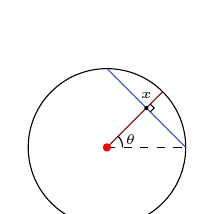
\begin{tikzpicture}
          \draw circle [radius = 1];
          \draw [mred] (0, 0) -- (0.707, 0.707);
          \draw [mblue] (0, 1) -- (1, 0);
          \draw [dashed] (0, 0) -- (1, 0);
          \node [circ, fill=red] at (0, 0) {};
          \node [circ, fill=black, scale=0.5] at (0.5, 0.5) {};
          \node at (0.5, 0.5) [above] {{\tiny $x$}};
          \draw[fill=gray!30] (0.2,0) 
          arc[start angle=0, end angle=45, radius=0.2];
          \node at (0.3, 0.1) {{\tiny$\theta$}};
          \draw (0.55, 0.45) -- (0.6, 0.5) -- (0.55, 0.55);
        \end{tikzpicture}
    \end{center}
    The corresponding sample space is
    \[
      \Omega = \set{(\theta, x)}{ \theta \in [0, 2 \pi),\, x \in [0,1]}.
    \]
    Because we choose the angle and radius uniformly on their respective
    intervals, and independently, we see that for any 
    $[a,b] \times [c,d] \subset [0, 2 \pi) \times [0,1]$ that
    \[
      \Prob([a,b] \times [c,d]) = \frac{b-a}{2 \pi} \cdot (d-c).
    \]
    Define a random variable
    \[
      X\left((\theta, x)\right) = \text{the length of the chord corresponding
      to the pair $(\theta, x)$} = 2 \sqrt{1 - x^2}.
    \]
    Now we see that
    \[
      \Prob\left(X \geq \sqrt{3}\right) = 
      \Prob([0,2 \pi] \times [0,1/2]) =
      \frac{2 \pi-0}{2 \pi} \cdot (1/2-0) =
      \frac{1}{2}
    \]
  
  \subsection{Second Solution}
    Now in order to choose a chord, we choose an arbitrary point inside
    the circle, and consider the chord perpendicular to the radius that is
    intersecting the with the point.
    \begin{center}
        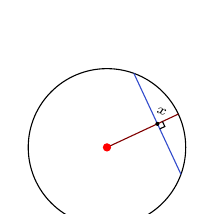
\begin{tikzpicture}
          \draw circle [radius = 1];
          \draw [mred, rotate=-20] (0, 0) -- (0.707, 0.707);
          \draw [mblue, rotate=-20] (0, 1) -- (1, 0);
          \node [circ, fill=red] at (0, 0) {};
          \node [circ, fill=black, scale=0.5] at 
          ([rotate around={-20:(0, 0)}] 0.5, 0.5) {};
          \node[rotate=-20] at ([rotate around={-20:(0, 0)}]0.5, 0.5) 
          [above] {{\tiny $x$}};
          \draw[rotate=-20] (0.55, 0.45) -- (0.6, 0.5) -- (0.55, 0.55);
        \end{tikzpicture}
    \end{center}
    The corresponding sample space is
    \[
      \Omega = \set{(x, y)}{ x^2 + y^2 \le 1}.
    \]
    Because we choose the coordinates uniformly, and independently, 
    we see that for any
    $[a,b] \times [c,d] \subset \Omega$ that
    \[
      \Prob([a,b] \times [c,d]) = \frac{(b-a)(d-c)}{\pi},
    \]
    which is just the area of the rectangle divided by the area of the circle.
    Define a random variable
    \[
      Y\left((x, y)\right) = \text{the length of the chord corresponding
      to the pair $(x, y)$} = 2 \sqrt{1 - x^2 - y^2}.
    \]
    Now we see that
    \[
      \Prob\left(Y \geq \sqrt{3}\right) = 
      \Prob\left(\set{(x,y)}{2 \sqrt{1 - x^2 - y^2} \geq \sqrt{3}}\right) =
      \Prob\left(\set{(x,y)}{x^2 + y^2 \le \frac{1}{4}}\right) =
      \frac{\frac{\pi}{4}}{\pi} =
      \frac{1}{4}
    \]
  \subsection{Third Solution}
    Now we simply choose a chord by choosing two points on the circle, and
    connecting them.
    \begin{center}
          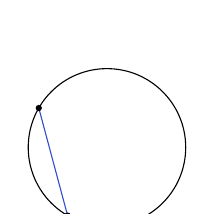
\begin{tikzpicture}
            \draw circle [radius = 1];
            \draw [mblue, rotate=-30] (0, -1) -- (-1, 0);
            \node [circ, fill=black, scale=0.75] at ([rotate=-30]-1, 0) {};
            \node [circ, fill=black, scale=0.75] at ([rotate=-30]0, -1) {};
          \end{tikzpicture}
    \end{center}
    The corresponding sample space is
    \[
      \Omega = \set{(\theta_1, \theta_2)}{\theta_1, \theta_2 \in [0,2 \pi)}.
    \]
    Because we choose the angles uniformly, and independently,
    we see that for any
    $[a,b] \times [c,d] \subset \Omega$ that
    \[
      \Prob([a,b] \times [c,d]) =
      \frac{b-a}{2 \pi} \cdot \frac{d-c}{2 \pi},
    \]
    Define a random variable
    \[
      Z\left((\theta_1, \theta_2)\right) = 
      \text{the length of the chord corresponding to the pair $(x, y)$}
    \]
    As you should expect, calculating $Z$ directly this time requires
    tedius geometric and trigonometric calculations.
    In the end of these calculations, we use similar methods to the ones
    shown in the first two solutions, and get
    \[
      \Prob\left(Z \geq \sqrt{3}\right) = 
      \frac{1}{3}
    \]

  \newpage

  \section{Multivariate Random Variables}
  \begin{definition}[Multivariate random variable]
    Let $(\Omega, \mathcal F, \Prob)$ be a probability space.
    The function $\vec{X} = (X_1,\dots,X_N) \colon \Omega \to \R^N$ is said
    to be a multivariate random variable if for all $a_i < b_i$ for 
    $1 \le i \le N$ we have
    \[
      \vec{X}^{-1}\left(\prod_{i=1}^{N} (a_i, b_i)\right) =
      \set{\omega \in \Omega}
      {a_i < X_i(\omega) < b_i,\, \forall 1 \le i \le N} \in
      \mathcal F.
    \]
    A multivariate random variable is sometimes also called a random vector.
  \end{definition}
  
  Notice that this definition also implies that $X^{-1}(A) \in \mathcal F$
  for all $A \in \mathfrak B\left(\R^n\right)$.

  \begin{proposition}
    Let $(\Omega, \mathcal F, \Prob)$ be a probability space, 
    and let $\vec{X} = (X_1,\dots,X_N) \colon \Omega \to \R^N$. 
    Then $\vec{X}$ is a multivariate random variable if and only if 
    $X_k \colon \Omega \to \R$ is a random variable for all $1 \le k \le N$.
  \end{proposition}
  \begin{proof}
    Assume $\vec{X}$ is a multivariate random variable and set some $1 \le k \le N$.
    Then for all $a < b$ we have
    \[
      X_k^{-1}((a,b)) = 
      \vec{X}^{-1}\left(\R^{k-1} \times (a,b) \times \R^{n-k}\right) \in
      \mathcal F.
    \]
    Now assume $X_1,\dots,X_N$ are random variables. Then for all $a_i < b_i$
    for $1 \le i \le N$ we have
    \[
      \vec{X}^{-1}\left(\prod_{i=1}^{N} (a_i, b_i)\right) =
      \bigcap_{i=1}^{N}\set{\omega \in \Omega}{a_i < X_i(\omega) < b_i} \in
      \mathcal F,
    \]
    where the last equality follows from the fact $\mathcal F$ is  sigma
    algebra, and $X_1,\dots,X_N$ are all random variables.
  \end{proof}

  \begin{definition}[Distribution of a multivariate random variable]
    Let $(\Omega, \mathcal F, \Prob)$ be a probability space, 
    and let $\vec{X} = (X_1,\dots,X_N) \colon \Omega \to \R^N$ be a multivariate
    random variable.
    The distribution of $\vec{X}$, denoted $\Prob_{\vec{X}}$ is a probability function
    on the measurable space $(\R^N, \mathfrak B_N)$ defined as
    \[
      \Prob_{\vec{X}}(A) =
      \Prob(\vec{X} \in A), \quad
      \forall A \in \mathfrak  B_N.
    \]
  \end{definition}

  \begin{remark}
    The function $\Prob_{X_k}$ denotes the distribution of the random
    variable $X_k$ and is called the partial distribution of $X_k$.
    We see that the distribution $\Prob_{\vec{X}}$ of a random vector uniquely
    defines the partial distributions $\Prob_{X_1},\dots,\Prob_{X_N}$
    because
    \[
      \Prob_{X_k} =
      \Prob_{\vec{X}}\left(\R^{k-1} \times A \times \R^{N-k}\right),
      \quad \forall A \in \mathfrak B.
    \]
    The opposite, is not true.
  \end{remark}

  \begin{example}
    There are $3$ red balls, $4$ white balls and $5$ blue balls in a vase.
    Three balls are arbitrarily drawn out of the vase.
    Denote the number of red balls drawn $X$, and the number of white
    balls drawn $Y$. What is the probability of $(X,Y)$?

    We see that
    \[
      \Omega = \set{(i,j)}{i,j \geq 0,\, i + j < 3},
    \]
    where $i$ denotes the number of red balls drawn, and $j$ the number
    of white balls drawn. From combinatorial arguments we get
    \[
      \Prob_{(X,Y)}\left((i,j)\right) =
      \frac{\binom{3}{i}\binom{4}{j}\binom{5}{3-i-j}}{\binom{12}{3}}.
    \]
  \end{example}

  \begin{definition}[Cumulatice distribution function]
    Let $(\Omega, \mathcal F, \Prob)$ be a probability space, 
    and let $\vec{X} = (X_1,\dots,X_N) \colon \Omega \to \R^N$ be a random vector.
    The cumulative ditribution function of $\vec{X}$, denoted $F_{\vec{X}}$, 
    is the function $F_{\vec{X}} \colon \R^N \to [0,1]$ defined as
    \[
      F_{\vec{X}}(a_1,\dots,a_N) =
      \Prob(X_i \le a_i,\, \forall 1 \le i \le N) =
      \Prob_{\vec{X}}\left(\prod_{i=1}^{N}(-\infty,a_i]\right).
    \]
  \end{definition}

  \begin{proposition}[Properties of the CDF]
    \begin{enumerate}
      \item The function $F_{\vec{X}}$ is increasing in each coordinate.
      \item The function $F_{\vec{X}}$ is continuous from the right in each 
        coordinate.
      \item For every choice $a_1,\dots,a_{k-1},a_{k+1},\dots,a_N \in \R$
        we have $\lim_{a_k \to -\infty}{F_X(a_1,a_2,\dots,a_N)} = 0$
      \item Denote $X^k = (X_1,\dots,X_{k-1},X_{k+1},\dots,X_N)$ the random 
      vector with the $k$-th coordinate erased. 
      Then for every choice $a_1,\dots,a_{k-1},a_{k+1},\dots,a_N \in \R$
      we have
      \[
        \lim_{a_k \to \infty} F_{\vec{X}}(a_1,a_2,\dots,a_N) =
        F_{X^k}(a_1,\dots,a_{k-1},a_{k+1},\dots,a_N).
      \]
      In particular
      \[
        \lim_{a_1,\dots,a_N \to \infty} F_{\vec{X}}(a_1,a_2,\dots,a_N) = 1.
      \]
    \end{enumerate}
  \end{proposition}
  \begin{proof}
    To be added.
  \end{proof}

  \begin{theorem}
    Every CDF corresponds to a unique distribution. In other words, if
    $(\Omega, \mathcal F, \Prob)$ and $(\Omega', \mathcal F', \Prob')$
    are two probability spaces, and $\vec{X} \colon \Omega \to \R^N$,
    $\vec{Y} \colon \Omega' \to \R^N$ are two random variable, then
    \[
      F_{\vec{X}} = F_{\vec{Y}} \iff 
      \Prob_{\vec{X}} = \Prob_{\vec{Y}}
    \]
  \end{theorem}
  \begin{theorem}
    Let $F \colon \R^N \to [0,1]$ be a function that satisfies all $4$ basic
    properties of the CDF. Thus, exists a probability space 
    $(\Omega, \mathcal F, \Prob)$ and a random variable 
    $\vec{X} \colon \Omega \to \R^N$ such that $F_{\vec{X}} = F$.
  \end{theorem}
  We won't prove this theorem either, but using these two last theorems
  we can conclude that exists a bijection between all random variables'
  distributions and functions that satisfy the $4$ properties from above.

  \begin{definition}[Discrete random vector]
    Let $(\Omega, \mathcal F, \Prob)$ be a probability space, 
    and let $\vec{X} = (X_1,\dots,X_N) \colon \Omega \to \R^N$ be a random vector.
    Then $\vec{X}$ is said to be a discrete random vector if exists a countable
    set $B \subset \R^\N$ such that $\Prob(\vec{X} \in B) = 1$.
  \end{definition}

  \begin{proposition}
    Let $(\Omega, \mathcal F, \Prob)$ be a probability space, 
    and let $\vec{X} = (X_1,\dots,X_N) \colon \Omega \to \R^N$ be a random vector.
    Then $\vec{X}$ is a discrete random vector if and only if $X_k$ is a discrete
    random variable for all $1 \le k \le N$.
  \end{proposition}
  \begin{proof}
    Assume that $\vec{X} = (X_1,\dots,X_N)$ is a discrete random vector.
    Then exists a countable set $B \subset \R^N$ such that
    \[
      \Prob_{\vec{X}}(B) = 1.
    \]
    Let $1 \le k \le N$. Consider the set $B_k = \pi_k(B)$ where $\pi_k$ is the
    projection on the $k$-th coordinate. It is clear that $B_k$ is countable
    and also
    \[
      1 \geq
      \Prob(X_1 \in B_k) =
      \Prob\left((X_1,X_2) \in B_k \times \R\right) \geq
      \Prob(\vec{X} \in B) =
      1.
    \]
    Thus we got that for all $1 \le k \le N$ that $X_k$ is discrete.
    Now suppose that $X_1,\dots,X_N$ are discrete random variables.
    Then exist countable sets $B_1,\dots,B_N$ such that 
    $\mathbf (X_k \in B_k) = 1$ for all $1 \le k \le N$.
    Under the axiom of choice we have that the set 
    $B = B_1 \times \cdots \times B_N$ is countable and it is clear that
    $\Prob(\vec{X} \in B) = 1$ as wanted which completes the proof.
  \end{proof}
  
  \begin{remark}
    Notice that the above proposition proves that given a discrete random
    vector $\vec{X} = (A_i)_{i=1}^{N}$, for any subsequence $\{i_j\}_{j=1}^{k}$ of 
    $\{i\}_{i=1}^N$ that $\vec{X} = (A_{i_j})_{j=1}^k$ is also a discrete random
    vector.
  \end{remark}

  \begin{definition}[Continuous random vector]
    Let $(\Omega, \mathcal F, \Prob)$ be a probability space, 
    and let $\vec{X} = (X_1,\dots,X_N) \colon \Omega \to \R^N$ be a random vector.
    Then $\vec{X}$ is called an absolutely continuous random vector if 
    $F_{\vec{X}}$ is continuous.
  \end{definition}
  
  \begin{remark}
    As in the case of a random variable, if $\vec{X} \colon \Omega \to \R^N$ is
    an absolutely continuous random vector, 
    then $\Prob(\vec{X} = a) = 0$ for all $a \in \R^N$.
  \end{remark}
  
  Similarly to general continuous random variables, we won't discuss
  general continuous random vectors in this course, and only consider
  absolutely continuous random vectors.

  \begin{definition}[Absolutely continuous random vector]
    Let $(\Omega, \mathcal F, \Prob)$ be a probability space, 
    and let $\vec{X} = (X_1,\dots,X_N) \colon \Omega \to \R^N$ be a random vector.
    Then $\vec{X}$ is said to be absolutely continuous if exists an integrable 
    function $f \colon \R^N \to [0,\infty)$ such that 
    \[
      \int_{\R_N} f(x)\,dx = 1
    \]
    And for all $a \in \R^N$
    \[
      F_{\vec{X}}(a) = 
      \Prob_{\vec{X}}\left(\prod_{i=1}^{N} (-\infty,a_i]\right) =
      \int_{\prod_{i=1}^{N} (-\infty,a_i]} f(y_1,\dots,y_N)\,d(y_1,\dots,y_N)).
    \]
    In this case, we call $f_{\vec{X}}$ the probability density function of 
    $\vec{X}$, or PDF for short.
  \end{definition}

  \begin{remark}
    Like in the case of random variables we konw that for any $A \subset \R^N$
    such that $f \cdot \mathbbm{1}$ is an integrable function
    \[
      \Prob_{\vec{X}}(A) = 
      \int_{A} f(y_1,\dots,y_N)\,d(y_1,\dots,y_N)).
    \]
  \end{remark}

  \begin{theorem}[Fubini's theorem]
    Let $f \colon A \times B \to \R$ be Riemann integrable, where 
    $A,B \subset \R$ are closed sets.
    For all $x \in A$ define the function $f_x \colon B \to \R$ by
    $f_x(y) = f(x,y)$.
    If for all $x \in A$ the function $f_x$ is Riemann integrable on $B$
    then
    \[
      \int_{A \times B} f(x,y)\,d(x,y) =
      \int_{A}\left(\int_{B} f_x(y)\,dy\right)
    \]
    Similarly, for each $y \in B$ we define the function 
    $f^y \colon A \to \R$ by $f^y(x) = f(x,y)$.
    If for all $y \in B$ the function $f^y$ is Riemann integrable on $A$
    then
    \[
      \int_{A \times B} f(x,y)\,d(x,y) =
      \int_{B}\left(\int_{A} f^y(x)\,dx\right)
    \]
  \end{theorem}
  \begin{example}
    Let $(X,Y)$ be a random vector with a probability density function
    defined as
    \[
      f_{(X,Y)}(x,y) =
      \begin{cases}
        c(2x+y^2), & 0 \le x \le 1, 0 \le y \le 2 \\
        0, &\text{otherwise}
      \end{cases}.
    \]
    Find the value of $c$, and calculate $\Prob(X + Y \le 1)$.

    To find $c$ we can use the fact that 
    $\int_{\R^2} f_{(X,Y)}(x,y)\,d(x,y) = 1$.
    From Fubini's thoerem
    \begin{align*}
      1 &= \int_{\R^2} f_{(X,Y)}(x,y)\,d(x,y) \\
      &= \int_{0}^{1}\left(\int_{0}^{2} c(2x + y^2)\,dy\right)\,dx \\
      &= c \int_{0}^{1} \left[2xy + \frac{y^3}{3}\right]\biggr\vert^2_0\,dx \\
      &= c \int_{0}^{1} 4x + \frac{8}{3}\,dx \\
      &= \frac{14}{3}c,
    \end{align*}
    which implies that $c = \frac{3}{14}$.

    To find $\Prob(X + Y \le 1)$, we need to understand that the function
    is only different than zero on $R = [0,1] \times [0,2]$. Which means that
    we need to find the integral of $f_X$ on 
    $T = R \cup \set{(x,y)}{x + y \le 1}$. 
    Using Fubini's theorem we get
    \begin{align*}
      \Prob(X + Y \le 1) &= \int_{T}f_{(X,Y)}*(x,y)\,d(x,y) \\
      &= \frac{3}{14} \int_{0}^{1} 
      \left(\int_{0}^{1-x} 2x + y^2\,dy\right)\,dx \\
      &= {\frac{3}{14}}\int_{0}^{1}2x(1-x)+{\frac{(1-x)^{3}}{3}}\,dx \\
      &= {\frac{5}{56}}.
    \end{align*}
  \end{example}

  \begin{theorem}\label{thm:randvec}
    Let $(\Omega, \mathcal F, \Prob)$ be a probability space, 
    and let $\vec{X} = (X_1,\dots,X_N) \colon \Omega \to \R^N$ be an absolutely
    continuous random vector with a probability density function 
    $f_{\vec{X}} \colon \R^N \to [0,\infty)$.
    Then $X_k$ is an absolutely continuous random variable for each
    $1 \le k \le N$, with a probability density function
    \[
      f_{X_{k}}(a) = 
      \int_{\R^{N-1}} 
      f_{\vec{X}}(x_{1},\dots,x_{k-1},a,x_{k+1},\dots,x_{N})
      d(x_{1},\ldots,x_{k-1},x_{k+1},\dots,x_{N}).
    \]
    And the same is true for other sub random vectors.
  \end{theorem}
  \begin{proof}
    To be added.
  \end{proof}
  
  \begin{definition}[Volume]
    Let $A \subset \R^N$ be a set. We define the volume of $A$ as such
    \[
      \Vol(B) = \int_{\R^N} \mathbbm{1}_B(x)\,dx
    \]
  \end{definition}
  
  \begin{definition}[Uniform distribution]
    Let $\vec{X} \colon \Omega \to \R^N$ be a random vector, 
    and $B \subset \R^N$ an open or closed set with a well defined, finite volume.
    The random vector $\vec{X}$ is said to distribute uniformly on $B$, and
    denote $\vec{X} \sim U(B)$ if $\vec{X}$ is absolutely continuous with a 
    density function
    \[
      f_{\vec{X}}(x) =
      \begin{cases}
        \frac{1}{\Vol(B)}, &x \in B \\
        0, &\text{otherwise}
      \end{cases}.
    \]
  \end{definition}

  A theorem needs to be here.

  \begin{definition}[Independence]
    Let $X_1,\dots,X_N \colon \Omega \to \R$ be random variables.
    The variables $X_1,\dots,X_N$ are said to be independent if
    for all $A_1,\dots,A_N \in \mathfrak B$ we have
    \[
      \Prob(X_1 \in A_1, \dots, X_N \in A_N) =
      \prod_{i=1}^{N} \Prob(X_i \in A_i).
    \]
  \end{definition}

  Notes and Examples
  
  \begin{definition}[Measure]
    Let $(X, \Sigma)$ be a measurable space.
    A set function $\mu \to [0,\infty]$ is called a measure if the following
    conditions hold
    \begin{enumerate}
      \item $\mu(\emptyset) = 0$;
      \item For all countable collections $\{E_{k}\}_{k=1}^{\infty }$ of
            pairwise disjoint sets in $\Sigma$
            \[ \mu \left(\bigcup _{k=1}^{\infty }E_{k}\right) =
               \sum _{k=1}^{\infty }\mu (E_{k}). \]
    \end{enumerate}
    The second condition is called $\sigma$-additivity.
  \end{definition}
  \begin{definition}[Atom]
    Given a measurable space $(X, \Sigma)$, and a measure $\mu$ on that
    space, a set $A \subset X$ in $\Sigma$ is called an atom if
    $\mu (A)>0$ and if for any measurable subset $B \subset A$ then
    $0\in \{\mu (B),\mu (A\setminus B)\}.$
  \end{definition}
  
  Mixed random vectors.

  \begin{definition}[Convolution]
    Let $f,g \colon \R \to [0,\infty)$. (In fact we can also use this 
    definition for $f,g \colon \R \to \R$ such that $\abs{f},\abs{g}$
    are integrable). The convolution of $f$ and $g$, denoted
    $f * g \colon \R \to [0,\infty)$ is the function
    \[
      (f * g)(a) = \int_{\R}f(x)g(a-x)\,dx.
    \]
  \end{definition}
  This is still missing a proof but
  \[
    F_{X+Y} = f_X * F_Y = f_Y * F_X.
  \]
  And
  \[
    f_{X+Y} = f_X * f_Y.
  \]

  \newpage

  \section{Expectation, Covariance and Correlation}
  A natural extension of expectation to random vectors is to set
  \[
    \E[\vec{X}] =
    \int_{\R^N} y f_{\vec{X}}(y)dy =
    \int_{\mathbb{R}^{N}} 
    \left(y_{1},\cdots,y_{N}\right)
    f_{\vec{X}} (y_{1},\cdot\cdot\cdot,y_{N})
    d(y_{1},\cdot\cdot\cdot\cdot,y_{N}).
  \]
  Recall that an intergal of vectors is defined as the vector of the
  integrals
  \[
    \E[\vec{X}] =
    \left(
    \int_{\mathbb{R}^{N}} 
    y_1 f_{\vec{X}} (y_{1},\cdot\cdot\cdot,y_{N})
    d(y_{1},\cdot\cdot\cdot\cdot,y_{N})
    ,\dots,
    \int_{\mathbb{R}^{N}} 
    y_N f_{\vec{X}} (y_{1},\cdot\cdot\cdot,y_{N})
    d(y_{1},\cdot\cdot\cdot\cdot,y_{N})
    \right).
  \]
  Now we can consider the first coordinate and using Fubini's theorem we
  get
  \begin{align*}
    \int_{\mathbb{R}^{N}} 
    y_1 f_{\vec{X}} (y_{1},\cdot\cdot\cdot,y_{N})
    d(y_{1},\cdot\cdot\cdot\cdot,y_{N}) &=
    \int_{\mathbb{R}}
    \left[\int_{\mathbb{R}^{N-1}}
    y_{1}f_{\vec{X}}(y_{1},\dots,y_{N}) d(y_{2},\dots, y_{N})\right]\,dy_{1} \\
    &= \int_{\mathbb{R}} y_1
    \left[\int_{\mathbb{R}^{N-1}}
    f_{\vec{X}}(y_{1},\dots,y_{N}) d(y_{2},\dots, y_{N})\right]\,dy_{1} \\
    &= \int_{\mathbb{R}} y_1
    f_{X_1}(y_1)\,dy_1 \\
    &= \E[X_1],
  \end{align*}
  where the last equality is from \autoref{thm:randvec}.
  This leads us to the following definition.
  \begin{definition}
    Let $\vec{X} \colon \Omega \to \R^N$ be a random vector such
    that $\E[X_i]$ is well defined and finite for all $1 \le i \le N$.
    Then we define
    \[
      \E[X] = (\E[X_1],\dots,\E[X_n]).
    \]
  \end{definition}

  \begin{proposition}
    Let $\vec{X} \colon \Omega \to \R^N$ be a random vector, and let
    $h \colon \R^N \to \R$ be a measurable function such that the
    random variable $\abs{h(\vec{X})}$ has a finite expectation.
    Then if $\vec{X}$ is absolutely continuous with a probability density
    function $f_{\vec{X}}$, then
    \[
      \E[h(\vec{X})] =
      \int_{\R^N} h(\vec{y}) f_{\vec{X}}(\vec{y})\,d\vec{y}.
    \]
    And if $\vec{X}$ is a discrete random vector with
    $\supp(\vec{X}) = (\vec{a}^i)_{i \geq 1}$, then
    \[
      \E[h(\vec{X})] =
      \sum_{i=1}^{\infty} h(\vec{a}^i) \Prob_{\vec{X}}(\vec{a}^i).
    \]
  \end{proposition}
  \begin{proof}
    To be added, possibly.
  \end{proof}

  \begin{corollary}[Linearity of Expectation]
    Let $X,Y \colon \Omega \to \R$ be two random variables and $a,b \in \R$.
    Then
    \[
      \E[aX + bY] = a \E[X] + b \E[Y].
    \]
  \end{corollary}

  \begin{corollary}
    Let $X,Y \colon \Omega \to \R$ be two random variables.
    If $X$ and $Y$ are independent then
    \[
      \E[XY] = \E[X] \E[Y].
    \]
    This implies
    \[
      \Var(X + Y) = \Var(X) + \Var(Y).
    \]
    But the converse is not always true.
  \end{corollary}

  For now, we won't write the proofs but here's a counter example to
  the previous direction of the above corollary.

  \begin{example}
    Let $X \sim U([-1,1])$ and $Y = X^2$. It is clear that $X$ and $Y$
    are not independent, but we have
    \[
      \E[XY] =
      \E[X^3] =
      \int_{-1}^{1} \frac{1}{2} x^3\,dx =
      0,
    \]
    but since $\E[X] = 0$, we get that
    \[
      \E[XY] = \E[X] \E[Y].
    \]
    and thus immediately
    \[
      \Var(X + Y) = \Var(X) + \Var(Y).
    \]
  \end{example}

  \begin{definition}[Uncorrelatedness]
    Two random vectors $X,Y \colon \Omega \to \R$ are said to be
    uncorrelated if $\E[XY] = \E[X] \E[Y]$.
  \end{definition}

  It is clear that if $X$, $Y$ are two independent random variables, then
  they are uncorrelated, but as we saw, the converse is not always true.

  A general formula that follows directely from the definition of variance
  and the linearity of expectation is
  \[
    \Var(X + Y) =
    \Var(X) + 
    2 \E \left[ (X - \E[X])(Y - \E[Y]) \right] +
    \Var(Y).
  \]
  Another such formula is
  \[
    \E \left[(X - \E[X])(Y - \E[Y])\right] =
    \E[XY] - \E[X] - \E[Y].
  \]

  Intuitively, the last value represents how dependent $X$, and $Y$ are.
  The farther it is from zero, the variables are less independent.
  Because it has multiple uses, we give it a special name.

  \begin{definition}(Covariance)
    Let $X,Y \colon \Omega \to \R$ be two random variables.
    The covariance of $X$ and $Y$, denoted $\Cov(X,Y)$ is defined
    as
    \[
      \Cov(X,Y) =
      \E \left[(X - \E[X])(Y - \E[Y])\right] =
      \E[XY] - \E[X] - \E[Y].
    \]
  \end{definition}
  
  From the definition of covariance we get the following convenient formula:
  \[
    \Var(X + Y) = \Var(X) + 2 \Cov(X,Y) + \Var(Y).
  \]
  Additionaly, the variables $X$, $Y$ are uncorrelated if and only if
  $\Cov(X,Y) = 0$.

  \begin{definition}[Correlation]
    The correlation of $X$, $Y$ is denoted $\rho_{X,Y}$, and defined
    as such
    \[
      \rho_{X,Y} =
      \frac{\Cov(X,Y)}{\sqrt{\Var(X)\Var(Y)}}.
    \]
  \end{definition}

  \begin{example}
    Suppose we made $n \geq 2$ experiments such that the probability to
    get $1$ in the experiment is $p_1$, the probability to get $2$ it
    $p_2$, and the probability to get $3$ is $p_3 = 1 - p_1 - p_2$.
    We denote $X$ the number of times we got $1$, and $Y$ the number
    of times we got $2$ in the experiments. Intuitively, since as $X$
    increases there are less experiments to get $2$ in $Y$ should decrease.
    This should result in the covariance and correlation of $X$ and $Y$
    to be negative. Indeed, since $X \sim \Bin(n,p_1)$ and 
    $Y \sim \Bin(n,p_2)$ we get that
    \[
      \mathbf [X] = np_1 \quad \text{and} \quad
      \mathbf [Y] = np_2.
    \]
    We notice that
    \begin{align*}
      X &= \sum_{i=1}^{n} \mathbbm{1}_{\{\text{the result is $1$}\}} \\
      Y &= \sum_{i=1}^{n} \mathbbm{1}_{\{\text{the result is $2$}\}},
    \end{align*}
    so we get
    \begin{align*}
      \E[XY] &=
      \E\left[
      \left(\sum_{i=1}^{n} \mathbbm{1}_{\{\text{the result is $1$}\}}\right)
      \left(\sum_{i=1}^{n} \mathbbm{1}_{\{\text{the result is $2$}\}}\right)
      \right] \\
      &= \sum_{i,j=1}^{n} \E\left[
      \mathbbm{1}_{\{\text{the result is $1$}\}}
      \mathbbm{1}_{\{\text{the result is $2$}\}}
      \right].
    \end{align*}
    We see that if $i = j$ the result can't be $1$ and $2$ so the
    expression inside the expectancy is zero, and thus the expectancy
    is also zero. If $i \neq j$ then the events are independent and
    we get
    \begin{align*}
      \E\left[
      \mathbbm{1}_{\{\text{the $i$ result is $1$}\}}
      \mathbbm{1}_{\{\text{the $j$ result is $2$}\}}
      \right] &=
      \E\left[
      \mathbbm{1}_{\{\text{the $i$ result is $1$}\}}
      \right]
      \E\left[
      \mathbbm{1}_{\{\text{the $j$ result is $2$}\}}
      \right] \\
      &= 
      \Prob(\text{the $i$ result is $1$})
      \Prob(\text{the $j$ result is $2$}) = p_1p_2
    \end{align*}
    Since there are $n(n-1)$ pairs $(i,j)$ such that $i \neq j$ we get
    \[
      \E[XY] = n(n-1) p_1 p_2
    \]
    Thus
    \[
      \Cov(X,Y) =
      \E[XY] - \E[X] \E[Y] =
      n(n-1) p_1 p_2 - n p_1 \cdot n p_2 = -n p_1 p_2.
    \]
    Finally, because the variance of a binomial random variable is
    $np(1-p)$ we have that
    \[
      \rho_{X,Y} =
      \frac{\Cov(X,Y)}{\sqrt{\Var(X) \cdot \Var(Y)}} =
      \frac{-n p_1 p_2}{\sqrt{np_1(1-p_1)np_2(1-p_2)}} =
      - \sqrt{\frac{p_1 p_2}{(1 - p_1)(1 - p_2)}}.
    \]
  \end{example}

  \begin{proposition}[Properties of Covariance]
    Let $X,X_1,X_2,Y \colon \Omega \to \R$ be random variables and 
    $a, b \in \R$. Then
    \begin{enumerate}
      \item $\Cov(X,Y) = \Cov(Y,X)$.
      \item $\Cov(aX,Y) = a \Cov(X,Y)$.
      \item $\Cov(X_1 + X_2,Y) = \Cov(X_1,Y) + \Cov(X_2,Y)$.
      \item $\Cov(X,X) \geq 0$.
      \item $\Cov(X,X) = 0 \iff \Var(X) = 0 \iff 
              \Prob(X = \E[X]) = 1$ ($X$ is constant).
      \item $\Cov(X + a, Y + b) = \Cov(X,Y)$.1
    \end{enumerate}
  \end{proposition}
  \begin{proof}
    The proofs for all of these properties follow from the definitions
    of variance, covariance, or the linearity of expectation.
  \end{proof}

  Notice that all random variables on a certain probability space
  $(\Omega, \mathcal F, \Prob)$ forms a vector space. We can also
  notice that the only things that's preventing the map 
  $(X,Y) \mapsto \Cov(X,Y)$ from defining an inner product, is that
  exist random variables $X \neq 0$ such that $\Cov(X,X) = 0$.
  Notably, all the constant random variables that are different than
  $0$. There is a way to fix this, by requiring the expectations on
  all random variables to be $0$. Now we can define the space
  \[
    L_2(\Omega, \mathcal F, \Prob) =
    \set{X \colon \Omega \to \R}
    {X\text{ is a random variable}, \E[X] = 0, \Var(X) < \infty}
  \]
  coupled with the bilinear form $\ip{X}{Y} := \Cov(X,Y)$.
  Then, the space 
  $\left(L_2(\Omega, \mathcal F, \Prob), \ip{\cdot}{\cdot}\right)$
  is an inner product space, and moreover, it is a Hilbert space.
  By the Cauchy--Schwarz inequality we get that
  \[
    \abs{\Cov(X,Y)} =
    \abs{\ip{X}{Y}} \le
    \sqrt{\ip{X}{X}} \cdot \sqrt{\ip{Y}{Y}} =
    \sqrt{\Var(X)} \cdot \sqrt{\Var(Y)}
  \]
  for all $X,Y \in L_2(\Omega, \mathcal F, \Prob)$.
  In fact, this inequality holds for any two random variables.
  If $\Var(X) = \infty$ or $\Var(Y) = \infty$ it holds very triviallly,
  so we may assume $\Var(X),\Var(Y) < \infty$.
  In this case, we know that $X - \E[X]$ and $Y - \E[Y]$ are both
  vectors in $L_2(\Omega, \mathcal F, \Prob)$ and thus
  \begin{align*}
    \abs{\Cov(X,Y)} &= \abs{\Cov{X - \E[X]}{Y - \E[Y]}} \\
    &\le \sqrt{\Var(X - \E[X])} \cdot \sqrt{\Var(Y - \E[Y])} \\
    &= \sqrt{\Var(X)} \cdot \sqrt{\Var(Y)}
  \end{align*}

  \begin{remark}
    The lasts proposition shows that the correlation of two random variables
    gives values in the interval $[0,1]$. 
    That is, for any $X,Y \colon \Omega \to \R$ we have 
    $-1 \le \rho_{X,Y} \le 1$.
  \end{remark}
  
  \begin{proposition}
    Let $X,Y \colon \Omega \to \R$ be two random variables.
    Then $X$ and $Y$ are independent if and only if for all measurable
    $f,g \colon \R \to \R$ such that $f(X)$, $g(Y)$, $f(X)g(Y)$ are
    integrable
    \[
      \E[f(X)g(Y)] = \E[f(X)] \E[g(Y)].
    \]
  \end{proposition}
  \begin{proof}
    To be added.
  \end{proof}
  
  \begin{example}
    Let $X \sim \Bin(n,p)$. Since all the experiments are independent
    we get that $X = \sum_{i=1}^{n} X_i$ for $X_i \sim \Bin(1,p)$ for
    $1 \le i \le n$. From the linearity of expectation we have
    \[
      \E[X] =
      \E\left[\sum_{i=1}^{n} X_i\right] =
      \sum_{i=1}^{n} \E[X_i] =
      \sum_{i=1}^{n} p =
      np.
    \]
    Since the variables are independent we can also easily calculate
    the variance:
    \[
      \Var(X) =
      \Var\left(\sum_{i=1}^{n} X_i\right) =
      \sum_{i=1}^{n} \Var(X_i) =
      \sum_{i=1}^{n} p(1-p) =
      n p(1-p)
    \]
  \end{example}
  
  \begin{example}
    Let $\sigma \colon [n] \to [n]$ be a random permutation from $S_n$.
    Denote $X$ the number of permutations of $\sigma$. Find $\E[X]$.

    First we notice that
    \[
      X = \sum_{i=1}^{n} \mathbbm{1}_{i \text{ is a fixed point}}
    \]
    and thus
    \begin{align*}
      \E[X] &=
      \E\left[\sum_{i=1}^{n} \mathbbm{1}_{i \text{ is a fixed point}}\right] \\
      &= \sum_{i=1}^{n} \E[\mathbbm{1}_{i \text{ is a fixed point}}] \\
      &= \sum_{i=1}^{n} \Prob(i \text{ is a fixed point}) \\
      &= \sum_{i=1}^{n} \frac{(n-1)!}{n!} \\
      &= \sum_{i=1}^{n} \frac{1}{n} \\
      &= 1.
    \end{align*}
    This method of using indicators to find the expectation is very useful
    and is sometimes called the ``method of indicator''.
  \end{example}
  
  \newpage

  \section{Conditional Probability Function and Expectation}

  \begin{definition}[Conditional probability function]
    Let $X,Y \colon \Omega \to \R$ be two random variables and $a \in \R$
    such that $\Prob_X(a) > 0$. The conditional probability of $Y$ given
    that $X = a$ is denoted 
    $\Prob_{Y \mid X}(\cdot \mid a) \colon \mathfrak B \to \R$ and defined as
    \[
      \Prob_{Y \mid X}(B \mid a) =
      \Prob(Y \in B \mid X = a) =
      \frac{\Prob(Y \in B, X = a)}{\Prob(X = a)}
    \]
  \end{definition}
  
  Here are some properties of the conditional probability function
  \begin{enumerate}
    \item $\Prob_{Y \mid X}(\cdot \mid a)$ is a probability function.
    \item $\Prob_Y(b) = \sum_{a} \Prob_X(a) \Prob_{Y \mid X}(b \mid a)$
      for all $b \in \R$.
    \item If $\Prob_Y(b) > 0$, then
    \[
      \Prob_{Y \mid X}(a \mid b) =
      \frac{\Prob_{Y \mid X}(b \mid a) \Prob_X(a)}{\Prob_Y(b)}.
    \]
  \end{enumerate}
  
  \begin{example}
    Let $X$ be the number of successes in $N$ independent Bernoulli experiments
    with probability $p$ of success, such that $N \sim \Poi(\lambda)$.
    Find the distribution of $X$.

    We get that for $k \geq 0$
    \begin{align*}
      \Prob_X(k) &= \sum_{n=0}^{\infty} \Prob_N(n) \Prob_{X \mid N}(k \mid n) =
      \sum_{n=k}^{\infty} \Prob_N(n) \Prob_{X \mid N}(k \mid n) \\
      &= \sum_{n=k}^{\infty} e^{-\lambda} \frac{\lambda^n}{n!} \cdot
        \binom{n}{k} p^k (1-p)^{n-k} \\
      &= \frac{e^{-\lambda}}{k!} p^k \lambda^k 
        \sum_{n=k}^{\infty} \frac{\lambda^{n-k}}{(n-k)!}(1-p)^{n-k} \\
      &= \frac{e^{-\lambda}}{k!} p^k \lambda^k 
        \sum_{n=0}^{\infty} \frac{\lambda^{n}}{(n)!}(1-p)^{n}
      = \frac{e^{-\lambda}}{k!} p^k \lambda^k e^{\lambda(1-p)}
      = e^{-\lambda p} \frac{(\lambda p)^{k}}{k!}.
    \end{align*}
  \end{example}

  Add discussion about more than one variable

  \begin{definition}[Conditional expectation for an event]
    Let $X,Y \colon \Omega \to \R$ be two discrete random variables and
    $a \in \R$ such that $\Prob_X(a) > 0$. The condition expectation of
    $Y$ given that $X = a$ is
    \[
      \E[Y \mid X = a] = \sum_{b} b \Prob_{Y \mid X}(b \mid a).
    \]
  \end{definition}

  \begin{example}
    To be added.
  \end{example}

  \begin{definition}[Conditional expectation, discrete variables]
    Let $X,Y \colon \Omega \to \R$ be two discrete random variables.
    Suppose that $\supp(X) = \{a_i\}_{i \geq 1}$.
    The conditional expectation of $Y$ given $X$ is a random variable
    $\E[Y \mid X] \colon \Omega \to \R$ defined as
    \[
      \E[Y \mid X](\omega) =
      \begin{cases}
        \E[Y \mid X = a_1], &\text{if } X(\omega) = a_1 \\
        \E[Y \mid X = a_2], &\text{if } X(\omega) = a_2 \\
        \E[Y \mid X = a_3], &\text{if } X(\omega) = a_3 \\
        \vdots
      \end{cases}
    \]
  \end{definition}

  Here are some properties of conditional expectation
  \begin{enumerate}
    \item To be added
  \end{enumerate}

  More stuff

  \begin{definition}[Conditional PDF]
    a
  \end{definition}
  \begin{definition}[Conditional expectation, absolutely continuous variables]
    Let. 
  \end{definition}

  \newpage

  \section{Borel--Cantelli Lemmas}

  Let $(\Omega, \mathcal F, \Prob)$ be a probability space, and 
  $(A_n)_{n \geq 1}$ an event sequence in $\mathcal F$.
  We denote
  \[
    \limsup_{n \to \infty} A_n =
    \{\omega \in A_n\text{ infinitely often}\} =
    \{\omega \in A_n\text{ i.o.}\}.
  \]
  Similarly,
  \[
    \liminf_{n \to \infty} A_n =
    \{\omega \in A_n \text{ eventually}\}.
  \]
  It is clear that
  \[
    \liminf_{n \to \infty} A_n \subset \limsup_{n \to \infty} A_n.
  \]
  \begin{definition}
    Let $(A_n)_{n \geq 1}$ be an event sequence.
    Then $A_n$ is said to have a limit if
    \[
      \liminf_{n \to \infty} A_n = \limsup_{n \to \infty} A_n.
    \]
    In this case, we denote
    \[
      \lim_{n \to \infty} A_n =
      \liminf_{n \to \infty} A_n = \limsup_{n \to \infty} A_n.
    \]
  \end{definition}

  Here add examples.

  Using this definition can now generalize \autoref{thm:continuity-base}.
  \begin{theorem}[Continuity of the probability function]
  \label{thm:continuity}
    Let $(\Omega, \mathcal F, \Prob)$ be a probability space and
    $(A_n)_{n \geq 1}$ an event sequence in $\mathcal F$ such that
    $\lim_{n \to \infty} A_n$ exists. Then,
    \[
      \lim_{n \to \infty} \Prob(A_n) =
      \Prob\left(\lim_{n \to \infty} A_n\right).
    \]
  \end{theorem}
  
  To prove this theorem, we need the following lemma
  \begin{lemma}[Fatou's lemma]\label{lem:fatou}
    Let $(\Omega, \mathcal F, \Prob)$ be a probability space and
    $(A_n)_{n \geq 1}$ an event sequence in $\mathcal F$. Then
    \begin{enumerate}
      \item $\Prob\left(\liminf_{n \to \infty} A_n\right) \le
            \liminf_{n \to \infty} \Prob(A_n)$
      \item $\Prob\left(\limsup_{n \to \infty} A_n\right) \geq
            \limsup_{n \to \infty} \Prob(A_n)$
    \end{enumerate}
  \end{lemma}
  \begin{proof}
    later
  \end{proof}
  We will know prove \autoref{thm:continuity}.
  \begin{proof}
    Suppose that $\lim_{n \to \infty} A_n$ exists.
    In this case we get from Fatou's lemma that
    \[
      \limsup_{n \to \infty} \Prob(A_n) \le
      \Prob\left(\limsup_{n \to \infty} A_n\right) =
      \Prob\left(\lim_{n \to \infty} A_n\right) =
      \Prob\left(\liminf_{n \to \infty} A_n\right) \le
      \liminf_{n \to \infty} \Prob(A_n)
    \]
    As we know that $\left(\Prob(A_n)\right)_{n \geq 1}$ is a sequence of
    numbers such that
    \[
      \limsup_{n \to \infty} \Prob(A_n) \le \liminf_{n \to \infty} \Prob(A_n)
    \]
    we know that it must converge and from the squeeze theorem we get that
    \[
      \lim_{n \to \infty} \Prob(A_n) =
      \Prob\left(\lim_{n \to \infty} A_n\right).
    \]
    Which completes the proof.
  \end{proof}

  The lemmas of Borel and Cantelli discuss the probability of the
  event $\limsup_{n \to \infty} A_n$. First we notice that
  \[
    \left( \limsup_{n \to \infty} A_n \right)^c =
    \left(\bigcap_{k=1}^{\infty} \bigcup_{n=k}^{\infty} A_n\right)^c =
    \bigcup_{k=1}^{\infty} \bigcap_{n=k}^{\infty} A_n^c =
    \liminf_{n \to \infty} A_n^c,
  \]
  which implies that any results about $\limsup_{n \to \infty} A_n$ could
  be translated into results about $\liminf_{n \to \infty} A_n^c$.

  \begin{lemma}[Borel--Cantelli lemma]
    Let $(\Omega, \mathcal F, \Prob)$ be a probability space, and let 
    $(A_n)_{n \geq 1}$ be a sequence of events in $\mathcal F$. Then
    \[
      \sum_{n=1}^{\infty} \Prob(A_n) < \infty \implies
      \Prob(\limsup_{n \to \infty} A_n) = 0.
    \]
  \end{lemma}
  \begin{proof}
    For $k \geq 1$ we define the event
    \[
      G_k := \bigcup_{n=k}^{\infty} A_n.
    \]
    It is clear that the sequence $(G_k)_{k=1}^{\infty}$ is decreasing.
    We also notice that
    \[
      \bigcap_{k=1}^{\infty} G_k =
      \bigcap_{k=1}^{\infty} \bigcup_{n=k}^{\infty} A_n =
      \limsup_{n \to \infty} A_n.
    \]
    This implies that
    \[
      \Prob\left(\limsup_{n \to \infty} A_n\right) =
      \Prob\left(\bigcap_{k=1}^{\infty} G_k\right) =
      \lim_{k \to \infty} \Prob(G_k).
    \]
    By definition we have that
    \[
      \Prob(G_k) =
      \Prob\left(\bigcup_{n=k}^{\infty} A_n\right) \le
      \sum_{n=k}^{\infty} \Prob(A_n)
    \]
    Finally, we get that
    \[
      \Prob\left(\limsup_{n \to \infty} A_n\right) =
      \lim_{k \to \infty} \Prob(G_k) \le
      \lim_{k \to \infty} \sum_{n=k}^{\infty} \Prob(A_n) =
      0.
    \]
    Where the last equality follows from the assumption that
    $\sum_{n=1}^{\infty} \Prob(A_n) < \infty$.
    Because the probability of any event is nonnegative we get that
    \[
      \Prob\left(\limsup_{n \to \infty} A_n\right) = 0,
    \]
    which completes the proof.
  \end{proof}

  \begin{example}
    
  \end{example}

  \begin{lemma}[Second Borel-Cantelli lemma]
    Let $(\Omega, \mathcal F, \Prob)$ be a probability space, and let
    $(A_n)_{n \geq 1}$ be a sequence of independent events in $\mathcal F$.
    Then
    \[
      \sum_{n=1}^{\infty} \Prob(A_n) = \infty \implies
      \Prob\left(\limsup_{n \to \infty} A_n\right) = 1.
    \]
  \end{lemma}
  
  \begin{proof}
    To be added.
  \end{proof}

  \newpage
  
  \section{Convergence of Random Variables}
  We have always known that random variables are functions,
  and we already know what convergence could mean in terms of functions.
  Here are a few definitions for convergence of random variables.

  \begin{definition}[Convergence in probability]
    Let $(\Omega, \mathcal F, \Prob)$ be a probability space, and let
    $X,X_1,X_2,\dots \colon \Omega \to \R$ be random variables.
    The sequence $X_n$ is said to converge in probability to $X$ if
    for all $\epsilon > 0$ we have
    \[
      \lim_{n \to \infty}
      \Prob\left(\{\abs{X_n - X} > \epsilon\}\right) = 0.
    \]
    In this case we denote $X_n \xrightarrow{p} X$.
  \end{definition}

  \begin{definition}[Convergence in $L^p$]
    Let $(\Omega, \mathcal F, \Prob)$ be a probability space, and let
    $X$ and $(A_n)_{n \geq 1}n \geq 1$ be random variables in that space.
    Given $p \geq 1$, the sequence $X_n$ is said to converge in $L^p$
    if
    \[
      \lim_{n \to \infty} \E\left[\abs{X_n - X}^p\right] = 0.
    \]
    In this case we denote $X_n \xrightarrow{L^p} X$.
    We sometimes say that $X_n$ converges to $X$ in the $r$-th mean.
  \end{definition}
  



  \section{The Law of Large Numbers}

  \section{The Central Limit Theorem}


\end{document}
